\subsection{A separability criterion}

PROPOSITION 11. --- Suppose that K is of characteristic exponent p, and let E be an algebraic extension of K, generated by a set S. If E is separable over K, then \(\mathrm{E} = \mathrm{K}(S^{p^{n}})\) for all integers \(n \geqslant 0\) ; conversely if E is of finite degree over K and \(\mathrm{E} = \mathrm{K}(S^{p})\) , then E is separable over K.

The case \(p = 1\) is trivial by the Cor. of V, p.~37. Suppose from now on that \(p \neq 1\) .

By hypothesis E is algebraic over K and we have \(E = K(S)\) , hence

\[
\mathrm{K} \left(\mathrm{S} ^ {p}\right) = \mathrm{K} \left(\mathrm{E} ^ {p}\right) = \mathrm{K} \left[ \mathrm{E} ^ {p} \right] \quad \text { by   V,   p.18,   Cor.   1 }.
\]

If E is of finite degree over K, it is a separable extension of K if and only if it is an etale algebra over K; the Cor. of V, p.~35 shows that this happens if and only if \(E = K[E^{p}]\) .

Suppose now that E is separable and of infinite degree over K. Then \(K[E^{p}]\) is the union of the subrings \(K[E^{\prime p}]\) where \(E'\) ranges over the set of subextensions of E of finite degree over K; but such an extension \(E'\) is separable over K (V, p.~36, Prop. 1), whence \(E' = K[E^{\prime p}] \subset K[E^{p}]\) by what has been said; finally we have \(E = K[E^{p}]\) . By induction on \(n \geqslant 0\) , the relation \(E = K[E^{p}]\) implies that \(E = K[E^{p^{n}}]\) .

COROLLARY 1. --- Every algebraic extension of a perfect field is a perfect field.

Let K be a perfect field of characteristic exponent p, and let E be an algebraic extension of K. Then E is separable over K (V, p.~36, Prop. 2) whence \(\mathrm{E} = \mathrm{K}(E^{p})\) by Prop. 11; but we have \(K = K^{p} \subset E^{p}\) , hence \(\mathrm{E} = \mathrm{K}(E^{p}) = E^{p}\) , and so E is perfect.

COROLLARY 2 (Mac Lane). --- Let \(\bar{\mathbf{K}}\) be an algebraic closure of \(\mathbf{K}\) and \(\mathrm{K}^{p^{-\infty}}\) the perfect closure of \(\mathbf{K}\) in \(\bar{\mathbf{K}}\) . For a subextension \(\mathbf{E}\) of \(\bar{\mathbf{K}}\) to be separable over \(\mathbf{K}\) it is necessary and sufficient that it should be linearly disjoint from \(\mathrm{K}^{p^{-\infty}}\) over \(\mathbf{K}\) .

We can immediately reduce to the case where \([E:K]\) is finite. Let \((x_{i})_{i\in I}\) be a basis of E over K. For E to be linearly disjoint from \(K^{p^{-\infty}}\) it is necessary and sufficient that it should be so from \(K^{p^{-n}}\) for all \(n\geqslant0\) , and this just means that the relation \(\sum_{i\in I}x_{i}a_{i}^{p^{-n}}=0\) implies \(a_{i}=0\) for all \(i\in I\) , for any family

\((a_{i})_{i\in I}\) of elements of K. This in turn means that the family \((x_{i}^{p^{n}})_{i\in I}\) is free over K, or also that it is a basis of the vector space E over K. Put differently, E is linearly disjoint from \(\mathbf{K}^{p^{-n}}\) if and only if \(\mathrm{E} = \mathrm{K}(\mathrm{E}^{p^n})\) . Now it suffices to apply Prop. 11.

Remarks. --- 1) When E is algebraic and of infinite degree over K, the condition \(E = K(E^{p})\) does not always ensure that E is separable over K. For example, if K is imperfect and E is a perfect closure of K, then we have \(E = K(E^{p})\) but E is not a separable extension of K (V, p.~39, Cor. 3).

\begin{enumerate}
\def\labelenumi{\arabic{enumi})}
\setcounter{enumi}{1}
\tightlist
\item
  Let \(\mathbf{E}\) be a separable algebraic extension of a field \(\mathbf{K}\) of characteristic exponent \(p\) . Then we have \(\mathbf{E}^p \cap \mathbf{K} = \mathbf{K}^p\) (Cor. 2); therefore if \(\mathbf{E}\) is perfect, the same is true of \(\mathbf{K}\) .
\end{enumerate}

\subsection{The relative separable algebraic closure}

PROPOSITION 12. --- Let E be an extension of K and \(E_{s}\) the set of elements of E which are algebraic and separable over K. Then \(E_{s}\) is the largest subextension of E which is algebraic and separable over K.

By Prop. 6, a) (V, p.~39) every subextension of E which is algebraic and separable over K is contained in \(E_{s}\) . By Prop. 6, b) (loc. cit.) the extension \(\mathrm{K}(E_{s})\) of K is algebraic and separable, whence \(\mathrm{K}(E_{s}) \subset E_{s}\) and so \(\mathrm{K}(E_{s}) = E_{s}\) .

With the notation of the preceding proposition, \(E_{s}\) is called the relative separable (algebraic) closure of K in E. When K is perfect, \(E_{s}\) is the relative algebraic closure of K in E (V, p.~36, Prop. 2).

PROPOSITION 13. --- Let E be an algebraic extension of K and let \(E_{s}\) be the relative separable algebraic closure of K in E.

\begin{enumerate}
\def\labelenumi{\alph{enumi})}
\item
  E is a \(p\) -radical extension of \(\mathrm{E}_s\) .
\item
  If \(\mathbf{F}\) is a subextension of \(\mathbf{E}\) such that \(\mathbf{E}\) is \(p\) -radical over \(\mathbf{F}\) , then \(\mathbf{F} \supseteq \mathbf{E}_s\) .
\item
  \(\mathbf{E}_s\) is the unique subextension of \(\mathbf{E}\) which is separable over \(\mathbf{K}\) and over which \(\mathbf{E}\) is \(p\) -radical.
\end{enumerate}

It suffices to prove \(a\) ) in the case where \(\mathbf{K}\) is of characteristic \(p \neq 0\) . Let \(x\) be an element of \(\mathbf{E}\) and \(f\) its minimal polynomial over \(\mathbf{K}\) . There exists an integer \(m \geqslant 0\) such that \(f\) belongs to \(\mathbf{K}[\mathbf{X}^{p^m}]\) but not to \(\mathbf{K}[\mathbf{X}^{p^{m+1}}]\) ; in other words, we have \(f(\mathbf{X}) = g(\mathbf{X}^{p^m})\) with \(g \in \mathbf{K}[\mathbf{X}], g \notin \mathbf{K}[\mathbf{X}^p]\) . Since \(f\) is irreducible, the same is true of \(g\) , hence \(g\) is the minimal polynomial of \(x^{p^m}\) over \(\mathbf{K}\) . By \(V\) , p.~38, Prop. 4 and p.~39, Prop. 5 we thus have \(x^{p^m} \in \mathrm{E}_s\) , so \(\mathbf{E}\) is \(p\) -radical over \(\mathrm{E}_s\) .

Assume now the hypothesis \(b)\) and let \(x \in \mathrm{E}_s\) . Since \(x\) is separable over \(\mathbf{K}\) , it is so also over \(\mathrm{F}(\mathrm{V}, \mathrm{p.~39}, \mathrm{Cor.~2})\) , but since \(\mathrm{E}\) is \(p\) -radical over \(\mathrm{F}\) , \(x\) is also \(p\) -radical over \(\mathrm{F}\) , hence \(x \in \mathrm{F}(\mathrm{V}, \mathrm{p.~39}, \mathrm{Cor.~3})\) .

Finally c) follows from a) and b) and Prop. 12.

COROLLARY 1. --- Let E and K' be two extensions of K contained in the same extension of K. Suppose that E is algebraic over K and denote by \(E_{s}\) the relative separable algebraic closure of K in E. Then \(\mathrm{K}'(\mathrm{E}_{s})\) is the relative separable algebraic closure of \(K'\) in \(\mathrm{K}'(\mathrm{E})\) .

For \(\mathbf{K}^{\prime}(\mathbf{E}_{s})\) is a separable algebraic extension of \(K^{\prime}\) by Prop. 10 (V, p.~42); since E is p-radical over \(E_{s}\) , the extension \(\mathbf{K}^{\prime}(\mathbf{E})\) of \(\mathbf{K}^{\prime}(\mathbf{E}_{s})\) is p-radical (V, p.~25, Cor.). Now it suffices to apply Prop. 13.

COROLLARY 2. --- If E has finite degree over K, then \(E_{s} = \bigcap_{n \geqslant 0} K(E^{p^{n}})\) .

For each integer \(n \geqslant 0\) denote by \(F_n\) the subextension \(K(E^{p^n})\) of \(E\) . The sequence \((F_n)_{n \geqslant 0}\) of vector subspaces of \(E\) is descending and \(E\) is of finite dimension over \(K\) . Hence there exists an integer \(m \geqslant 0\) such that \(F_m = F_n\) for all \(n \geqslant m\) . We thus have \(K(F_m^p) = F_{m+1} = F_m\) , hence \(F_m\) is a separable extension of \(K(V, p. 42, \text{Prop. } 11)\) ; it is clear that \(E\) is \(p\) -radical over \(F_m\) and so Prop. 13 implies \(E_s = F_m = \bigcap_{n \geqslant 0} F_n\) .

Remark. --- Let E be an algebraic extension of K and \(E_{r}\) the relative p-radical closure of E in K (V, p.~25). Then \(E_{r}\) is the largest subextension of E which is p-radical over K (V, p.~25, Prop. 2). However, E is in general not separable over \(E_{r}\) (V, p.~152, Ex. 2); for the case of quasi-Galois extensions see V, p.~76.

\subsection{The separable closure of a field}

DEFINITION 4. --- A field K is said to be separably closed if every separable algebraic extension of K is trivial.

An algebraically closed field is separably closed. Conversely, if a perfect field K is separably closed, it is algebraically closed, because every algebraic extension of K is separable (V, p.~3, Prop. 2).

DEFINITION 5. --- Let K be a field. By a separable algebraic closure, or (by abuse of language) separable closure of K we understand any extension E of K which is algebraic and separable over K, and such that the field E is separably closed.

When K is perfect, there is complete identity between the notions of separable closure and algebraic closure of K (V, p.~36, Prop. 2 and p.~43, Cor. 1).

PROPOSITION 14. --- Let \(\Omega\) be an algebraically closed extension of K.

\begin{enumerate}
\def\labelenumi{\alph{enumi})}
\item
  The relative separable algebraic closure \(\Omega_s\) of \(\mathbf{K}\) in \(\Omega\) is a separable closure of \(\mathbf{K}\) .
\item
  If E and E' are two separable closures of K, there exists a K-isomorphism of E onto E'.
\end{enumerate}

Let \(F\) be a separable algebraic extension of \(\Omega_s\) ; since \(\Omega\) is algebraically closed, there exists an \(\Omega_s\) -homomorphism \(u\) of \(F\) into \(\Omega\) (V, p.~20, Th. 1). By Prop. 9 (V, p.~42) \(u(F)\) is separable over \(K\) , hence \(u(F) = \Omega_s\) . Therefore \(F\) is a trivial extension of \(\Omega_s\) and so \(\Omega_s\) is separably closed, whence \(a\) ).

Let E be a separable closure of K. Since E is an algebraic extension of K, there exists a K-homomorphism v of E into \(\Omega\) (V, p.~20, Th. 1). Hence \(v(\mathrm{E})\) is separable algebraic over K, whence \(v(\mathrm{E}) \subset \Omega_{s}\) . By V, p.~42, Prop. 9, \(\Omega_{s}\) is separable over \(v(\mathrm{E})\) and since the field \(v(\mathrm{E})\) is separably closed, we have \(v(\mathrm{E}) = \Omega_{s}\) . It follows that v is a K-isomorphism of E onto \(\Omega_{s}\) . Now b) is an immediate consequence.

COROLLARY. --- Let E be a separably closed extension of K and F a separable algebraic extension of K; then there exists a K-homomorphism of F into E.

Let \(\Omega\) be an algebraic closure of E; we have \(\Omega_s \subset E\) and it suffices to treat the case where \(E = \Omega_s\) . Since F is an algebraic extension of K, there exists a K-homomorphism \(u\) of F into \(\Omega\) (V, p.~20, Th. 1). Since the field \(u(F)\) is separable over K, we have \(u(F) \subset \Omega_s\) and \(u\) defines a K-homomorphism of F into \(\Omega_s = E\) .

\pandocbounded{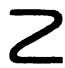
\includegraphics[keepaspectratio]{images/part001_42ca6df9.jpg}}

Remarks. --- 1) Let E and E' be two separable closures of K. If K is not separably closed, there exist several K-isomorphisms of E onto E'. For E is then a non-trivial Galois extension of K, and so there exist K-automorphisms of E distinct from the identity (V, p.~56, Th. 1).

2) Let \(E\) be an algebraic and separable extension of \(K\) . If every algebraic and separable extension of \(K\) is isomorphic to a subextension of \(E\) , then \(E\) is a separable closure of K. For if \(E'\) is a separable closure of K, then each of the extensions E and \(E'\) is isomorphic to a subextension of the other; hence E and \(E'\) are isomorphic extensions of K (V, p.~52, Prop. 1, a)).

\subsection{Separable and inseparable degrees of an extension of finite degree}

Let E be an extension of finite degree of K and \(\Omega\) an algebraic closure of K. Recall (V, p.~31) that by the separable degree of E over K, written \([E:K]_{s}\) , we understand the number of K-homomorphisms of E into \(\Omega\) .

PROPOSITION 15. --- Let \(\mathbf{E}_s\) be the relative separable closure of \(\mathbf{K}\) in \(\mathbf{E}\) ; then \([\mathbf{E}:\mathbf{K}]_s = [\mathbf{E}_s:\mathbf{K}]\) .

The field \(\Omega\) is perfect and \(E\) is \(p\) -radical over \(E_s\) , by \(V\) , p.~44, Prop. 13; therefore Prop. 3 (V, p.~26) shows that every K-homomorphism of \(E_s\) into \(\Omega\) extends in a unique fashion to a K-homomorphism of \(E\) into \(\Omega\) ; we thus have \([E:K]_s = [E_s:K]_s\) . Since \(E_s\) is a separable extension of finite degree of \(K\) , it is an etale algebra over \(K\) ; so we have \([E_s:K]_s = [E_s:K]\) by \(V\) , p.~32, Prop. 4, and the result follows.

With the preceding notation, the degree of E over \(E_{s}\) is called the inseparable degree of E over K and is denoted by \([E:K]_{i}\) . We thus have

\[
[ \mathrm{E}: \mathrm{K} ] = [ \mathrm{E}: \mathrm{K} ] _ {s} \cdot [ \mathrm{E}: \mathrm{K} ] _ {i}\tag{1}
\]

by Prop. 15.

\pandocbounded{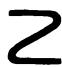
\includegraphics[keepaspectratio]{images/part001_fb7ec604.jpg}}

When K is of characteristic 0, then \(E = E_{s}\) , and so \([E : K]_{s} = [E : K]\) and \([E : K]_{i} = 1\) . If K is of characteristic \(p \neq 0\) , the number \([E : K]_{i}\) is a power of p because E is p-radical over \(E_{s}\) (V, p.~44, Prop. 13 and p.~26, Prop. 4). It should be noted that \([E : K]_{i}\) is not necessarily equal to the highest power of p dividing \([E : K]\) , nor equal to the degree \([E_{r} : K]\) of the relative p-radical closure of E in K (V, p.~152, Ex. 3 and 2).

PROPOSITION 16. --- Let \(\Omega\) be an extension of K and E, F two subextensions of \(\Omega\) , of finite degree over K.

\begin{enumerate}
\def\labelenumi{\alph{enumi})}
\item
  If \(\mathrm{E} \subset \mathrm{F}\) , then \([\mathrm{F}:\mathrm{K}]_s = [\mathrm{F}:\mathrm{E}]_s \cdot [\mathrm{E}:\mathrm{K}]_s\) and \([\mathrm{F}:\mathrm{K}]_i = [\mathrm{F}:\mathrm{E}]_i \cdot [\mathrm{E}:\mathrm{K}]_i\) .
\item
  Let \(\mathbf{K}'\) be a subextension of \(\Omega\) ; then we have
\end{enumerate}

\[
\left[ \mathrm{K} ^ {\prime} (\mathrm{E}): \mathrm{K} ^ {\prime} \right] _ {s} \leqslant \left[ \mathrm{E}: \mathrm{K} \right] _ {s} \quad \text{and} \quad \left[ \mathrm{K} ^ {\prime} (\mathrm{E}): \mathrm{K} ^ {\prime} \right] _ {i} \leqslant \left[ \mathrm{E}: \mathrm{K} \right] _ {i},
\]

and equality holds if \(\mathbf{K}'\) is linearly disjoint from \(\mathbf{E}\) over \(\mathbf{K}\) .

\begin{enumerate}
\def\labelenumi{\alph{enumi})}
\setcounter{enumi}{2}
\tightlist
\item
  We have \([\mathrm{K}(\mathrm{E}\cup \mathrm{F}):\mathrm{K}]_s\leqslant [\mathrm{E}:\mathrm{K}]_s.\) \([\mathrm{F}:\mathrm{K}]_s\) and \([\mathrm{K}(\mathrm{E}\cup \mathrm{F}):\mathrm{K}]_i\leqslant [\mathrm{E}:\mathrm{K}]_i.\) \([\mathrm{F}:\mathrm{K}]_i\) , and equality holds if E and F are linearly disjoint over K.
\end{enumerate}

The assertion about the separable degrees in \(a\) follows from (9) (V, p.~32). Since \([F:K] = [F:E].[E:K]\) , the assertion about the inseparable degrees follows from this and (1).

By Cor. 1 of Prop. 13 (V, p.~44) and Prop. 15, we have

\[
\left[ \mathrm{K} ^ {\prime} (\mathrm{E}): \mathrm{K} ^ {\prime} \right] _ {s} = \left[ \mathrm{K} ^ {\prime} \left(\mathrm{E} _ {s}\right): \mathrm{K} ^ {\prime} \right], \quad \left[ \mathrm{K} ^ {\prime} (\mathrm{E}): \mathrm{K} ^ {\prime} \right] _ {i} = \left[ \mathrm{F} ^ {\prime} (\mathrm{E}): \mathrm{K} ^ {\prime} \left(\mathrm{E} _ {s}\right) \right];\tag{2}
\]

when \(K'\) is linearly disjoint from E over K, then \(E_{s}\) is linearly disjoint from \(K'\) over K and E is linearly disjoint from \(\mathrm{K}'(\mathrm{E}_{s})\) over \(E_{s}\) (V, p.~15, Prop. 8). Assertion b) now follows from Prop. 5 (V, p.~14).

By a) we have \([\mathbf{K}(\mathbf{E}\cup\mathbf{F}):\mathbf{K}]_{s}=[\mathbf{F}(\mathbf{E}):\mathbf{F}]_{s}\cdot[\mathbf{F}:\mathbf{K}]_{s}\) ; by b) we have \([\mathbf{F}(\mathbf{E}):\mathbf{F}]_{s}\leqslant[\mathbf{E}:\mathbf{K}]_{s}\) with equality if E and F are linearly disjoint over K. Hence we obtain the inequality \([\mathbf{K}(\mathbf{E}\cup\mathbf{F}):\mathbf{K}]_{s}\leqslant[\mathbf{E}:\mathbf{K}]_{s}\cdot[\mathbf{F}:\mathbf{K}]_{s}\) with equality if E and F are linearly disjoint over K. The assertion of c) about the inseparable degrees is proved in a similar fashion.

\section{NORMS AND TRACES}

Throughout this paragraph K denotes a field.

\subsection{Recall}

Let A be an algebra of finite degree n over K. For each \(x \in A\) we denote by \(L_{x}\) the linear mapping \(a \mapsto xa\) of A into itself. We recall (III, p.~543) that the trace of \(L_{x}\) is called the trace of x relative to A and is written \(\operatorname{Tr}_{\mathbf{A}/\mathbf{K}}(x)\) ; likewise the determinant of \(L_{x}\) is called the norm of x relative to A and is denoted by \(\mathrm{N}_{\mathrm{A}/\mathrm{K}}(x)\) . The discriminant of a sequence \((x_{1}, \ldots, x_{n})\) of n elements of A is by definition the determinant \(\mathrm{D}_{\mathrm{A}/\mathrm{K}}(x_{1}, \ldots, x_{n})\) of the matrix \((\operatorname{Tr}_{\mathrm{A}/\mathrm{K}}(x_{i}x_{j}))_{1 \leq i,j \leq n}\) (III, p.~549).

Let \(\mathbf{K}'\) be an extension of \(\mathbf{K}\) and let \(\mathbf{A}' = \mathbf{A}_{(\mathbf{K}')}\) be the \(\mathbf{K}'\) -algebra derived from \(\mathbf{A}\) by extension of scalars. We have the formulae

\[
\operatorname{Tr} _ {\mathrm{A} ^ {\prime} / \mathrm{K} ^ {\prime}} (1 \otimes x) = \operatorname{Tr} _ {\mathrm{A} / \mathrm{K}} (x). 1, \quad \mathrm{N} _ {\mathrm{A} ^ {\prime} / \mathrm{K} ^ {\prime}} (1 \otimes x) = \mathrm{N} _ {\mathrm{A} / \mathrm{K}} (x). 1\tag{1}
\]

for all \(x \in \mathbf{A}\) (III, p.~544). For every sequence \((x_1, \ldots, x_n)\) of elements of \(\mathbf{A}\) we have

\[
\mathrm{D} _ {\mathrm{A} ^ {\prime} / \mathrm{K} ^ {\prime}} (1 \otimes x _ {1}, \dots , 1 \otimes x _ {n}) = \mathrm{D} _ {\mathrm{A} / \mathrm{K}} (x _ {1}, \dots , x _ {n}). 1,\tag{2}
\]

as follows from the first formula (1).

\subsection{Norms and traces in etale algebras}

Let A be an etale algebra of (finite) degree n over K. By definition there exist then an extension L of K and distinct homomorphisms \(u_{1}, \ldots, u_{n}\) of A into L with the following properties.

\begin{enumerate}
\def\labelenumi{\alph{enumi})}
\item
  every homomorphism of \(\mathbf{A}\) into \(\mathbf{L}\) is equal to one of the \(u_{i}\) (V, p.~29, Cor.)
\item
  there exists an L-algebra isomorphism \(u: \mathbf{A}_{(L)} \to L^n\) such that
\end{enumerate}

\[
u (1 \otimes x) = \left(u _ {1} (x), \dots , u _ {n} (x)\right) \quad \text { for   all } \quad x \in A.
\]

Moreover, every algebraically closed extension L of K has the above properties (V, p.~30, Prop. 2).

We fix \(L, u_1, \ldots, u_n\) in what follows. Let \(x \in A\) ; we shall prove the formulae

\[
\operatorname{Tr} _ {\mathrm{A} / \mathrm{K}} (x) \cdot 1 = \sum_ {i = 1} ^ {n} u _ {i} (x), \quad \mathrm{N} _ {\mathrm{A} / \mathrm{K}} (x) \cdot 1 = \prod_ {i = 1} ^ {n} u _ {i} (x).\tag{3}
\]

Let \(v\) be multiplication by \(1 \otimes x\) in \(\mathbf{A}_{(L)}\) ; with respect to the basis of \(\mathbf{A}_{(L)}\) which is the image under \(u^{-1}\) of the canonical basis of \(L^n\) , the matrix of the linear mapping \(v\) is diagonal, with diagonal elements \(u_1(x), \ldots, u_n(x)\) . We conclude that

\[
\operatorname{Tr} _ {\mathrm{A} _ {(\mathrm{L})} / \mathrm{L}} (1 \otimes x). 1 = \sum_ {i = 1} ^ {n} u _ {i} (x), \text { whence } \operatorname{Tr} _ {\mathrm{A} / \mathrm{K}} (x). 1 = \sum_ {i = 1} ^ {n} u _ {i} (x) \text { by } (1);
\]

the case of norms is treated similarly.

Further let \((x_{1},\ldots ,x_{n})\) be a sequence of elements of A, let U be the matrix

\[
\left(u _ {i} \left(x _ {j}\right)\right) _ {1 \leqslant i, j \leqslant n}
\]

and let \((t_{ij}) = {}^t\mathrm{U} \cdot U\) . By the first formula (3) we have

\[
\operatorname{Tr} _ {\mathrm{A} / \mathrm{K}} \left(x _ {i} x _ {j}\right) \cdot 1 = \sum_ {k = 1} ^ {n} u _ {k} \left(x _ {i} x _ {j}\right) = \sum_ {k = 1} ^ {n} u _ {k} \left(x _ {i}\right) u _ {k} \left(x _ {j}\right) = t _ {i j};
\]

passing to determinants, we obtain

\[
\mathrm{D} _ {\mathrm{A} / \mathrm{K}} (x _ {1}, \dots , x _ {n}) \cdot 1 = [ \det u _ {i} (x _ {j}) ] ^ {2}.\tag{4}
\]

PROPOSITION 1. --- Let A be a commutative algebra of finite degree over K. Then the following conditions are equivalent :

\begin{enumerate}
\def\labelenumi{\alph{enumi})}
\item
  The algebra \(\mathbf{A}\) is etale.
\item
  There exists a basis of \(\mathbf{A}\) whose discriminant is non-zero.
\item
  For each \(x \neq 0\) in A there exists \(y\) in A such that \(\operatorname{Tr}_{\mathbf{A} / \mathbf{K}}(xy) \neq 0\) .
\end{enumerate}

Further, when these conditions are satisfied, the discriminant of any basis of A is non-zero.

We shall show that when A is assumed etale, the discriminant of A with respect to any basis \((x_{1},\ldots,x_{n})\) of A over K is non-zero; this will in particular establish the implication \(a)\Rightarrow b)\) . By (4), with the above notation, it suffices to show that the matrix U is invertible, or equivalently, that the system of linear equations

\[
\sum_ {i = 1} ^ {n} \lambda_ {i} u _ {i} (x _ {j}) = 0 \quad (\text { for } 1 \leqslant j \leqslant n)\tag{5}
\]

has only the solution \(\lambda_{1} = \cdots = \lambda_{n} = 0\) in L. Now the relation (5) implies \(\sum_{i=1}^{n} \lambda_{i} u_{i}(x) = 0\) for all \(x \in \mathbf{A}\) , whence \(\lambda_{i} = 0\) for \(1 \leqslant i \leqslant n\) , by the theorem on the

linear independence of homomorphisms (V, p.~27, Th. 1).

The equivalence of \(b)\) and \(c)\) is a consequence of the following general lemma:

Lemma 1. --- Let V be a vector space of finite dimension over K and B a bilinear form on V × V. Let \((v_{1}, \ldots, v_{n})\) be a basis of V over K and \(\Delta = \det B(v_{i}, v_{j})\) . Then \(\Delta \neq 0\) if and only if, for each \(x \neq 0\) in V there exists y in V such that \(B(x, y) \neq 0\) .

We have \(\Delta \neq 0\) if and only if the system of linear equations

\[
\sum_ {i = 1} ^ {n} \lambda_ {i} \mathrm{B} (v _ {i}, v _ {j}) = 0 \quad (1 \leqslant j \leqslant n)
\]

has only the solution \(\lambda_1 = \cdots = \lambda_n = 0\) in K. If we put \(x = \sum_{i=1}^{n} \lambda_i v_i\) , the above system is equivalent to B \((x, v_j) = 0\) for \(1 \leqslant j \leqslant n\) , or also, since \((v_1, \ldots, v_n)\) is a basis of V over K, to B \((x, y) = 0\) for all \(y \in V\) , whence the lemma.

Let us show that condition c) implies that A is reduced. Let x be a nilpotent element of A; for any \(y \in A\) the element xy is nilpotent, and so the endomorphism \(L_{xy}\) of the vector space A is nilpotent. Now the following lemma implies that \(\operatorname{Tr}(xy) = 0\) for all \(y \in A\) , whence x = 0 under hypothesis c).

Lemma 2. --- Let V be a vector space of finite dimension over K and u a nilpotent endomorphism of V, then \(\operatorname{Tr}(u)=0\) .

For each integer \(n \geqslant 0\) let \(V_n\) be the image of \(u^n\) . Since \(u\) is nilpotent, there exists an integer \(r \geqslant 0\) such that \(V_0 = V\) , \(V_r = 0\) and \(V_i \neq V_{i+1}\) for \(0 \leqslant i \leqslant r-1\) . Let \(d_i\) be the dimension of \(V_{i-1}\) (for \(1 \leqslant i \leqslant r\) ). There exists a basis \((x_1, \ldots, x_d)\) of \(V\) such that the vectors \(x_j\) with \(d - d_i < j \leqslant d\) form a basis of \(V_{i-1}\) (for \(1 \leqslant i \leqslant r\) ). We have \(u(V_{i-1}) \subset V_i\) and so the diagonal elements of the matrix of \(u\) for the basis \((x_1, \ldots, x_d)\) are zero. Thus we have \(\operatorname{Tr}(u) = 0\) and the lemma follows.

Finally let us show that \(b)\) implies \(a)\) . Let \((x_1, \ldots, x_n)\) be a basis of \(A\) over \(K\) such that \(D_{A/K}(x_1, \ldots, x_n) \neq 0\) . Let \(K'\) be an extension of \(K\) , \(A'\) the \(K'\) -algebra derived from \(A\) by extension of scalars and \(x_i' = 1 \otimes x_i\) for \(1 \leqslant i \leqslant n\) . By Formula (2) (V, p.~47) we have \(D_{A'/K'}(x_1', \ldots, x_n') \neq 0\) . Applying the preceding result to \(A'\) we see that \(A'\) is reduced, hence the algebra \(A\) is etale (V, p.~34, Th. 4).

COROLLARY. --- Let E be an extension of finite degree of K. For E to be separable it is necessary and sufficient that there exist a in E such that \(\operatorname{Tr}_{E/K}(a) \neq 0\) .

The condition is necessary by Prop. 1. Conversely, assume that there exists \(a \in E\) such that \(\operatorname{Tr}_{E/K}(a) \neq 0\) . Given \(x \neq 0\) in \(E\) , if we put \(y = ax^{-1}\) , then \(\operatorname{Tr}_{E/K}(xy) \neq 0\) . Now Prop. 1 shows that \(E\) is an etale algebra over \(K\) , hence a separable extension of \(K\) .

\subsection{Norms and traces in extensions of finite degree}

The transitivity formulae in algebras (III, p.~548) imply the following proposition in the case of extensions of finite degree.

PROPOSITION 2. --- Let F be an extension of finite degree of K and E a subextension of F. Then for every \(x \in F\) we have

\[
\operatorname{Tr} _ {\mathrm{F} / \mathrm{K}} (x) = \operatorname{Tr} _ {\mathrm{E} / \mathrm{K}} (\operatorname{Tr} _ {\mathrm{F} / \mathrm{E}} (x))\tag{6}
\]

\[
\mathrm{N} _ {\mathrm{F} / \mathrm{K}} (x) = \mathrm{N} _ {\mathrm{E} / \mathrm{K}} (\mathrm{N} _ {\mathrm{F} / \mathrm{E}} (x))\tag{7}
\]

COROLLARY. --- Put \(m = [F : E]\) ; then for every \(x \in E\) we have

\[
\operatorname{Tr} _ {\mathrm{F} / \mathrm{K}} (x) = m. \operatorname{Tr} _ {\mathrm{E} / \mathrm{K}} (x)\tag{8}
\]

\[
\mathrm{N} _ {\mathrm{F} / \mathrm{K}} (x) = \mathrm{N} _ {\mathrm{E} / \mathrm{K}} (x) ^ {m}\tag{9}
\]

PROPOSITION 3. --- Let E be an extension of finite degree n of K and x an element of E, of degree d over K. Write \(f(X) = X^d + \sum_{i=1}^{d} a_i X^{d-i}\) for the minimal polynomial of x over K. Then we have

\[
\mathrm{Tr} _ {\mathrm{E/K}} (x) = - \frac {n}{d} a _ {1}\tag{10}
\]

\[
\mathrm{N} _ {\mathrm{E} / \mathrm{K}} (x) = ((- 1) ^ {d} a _ {d}) ^ {n / d} = (- 1) ^ {n} a _ {d} ^ {n / d}\tag{11}
\]

Prop. 3 follows directly from the Cor. of Prop. 2 and the lemma :

Lemma 3. --- Let R be a commutative ring, \(f(\mathbf{X}) = \mathbf{X}^d + \sum_{i=1}^{d} a_i \mathbf{X}^{d-i}\) a monic polynomial of R{[}X{]}, A the R-algebra R{[}X{]}/(f) and x the residue class of X in A. Then \(\operatorname{Tr}_{\mathrm{A/R}}(x) = -a_1\) and \(\mathrm{N}_{\mathrm{A/R}}(x) = (-1)^d a_d\) .

By the Cor. (IV, p.~11) the sequence \((1, x, \ldots, x^{d-1})\) is a basis of \(\mathbf{A}\) ; further we have

\[
\begin{array}{r l} x \cdot 1 = x, & x \cdot x = x ^ {2}, \dots , x \cdot x ^ {d - 2} = x ^ {d - 1}, \\ & x \cdot x ^ {d - 1} = - a _ {d} \cdot 1 - a _ {d - 1} \cdot x - \dots - a _ {1} \cdot x ^ {d - 1}. \end{array}
\]

The matrix which expresses the multiplication by x with respect to the basis \((1, x, \ldots, x^{d-1})\) of A is thus of the following form (we have taken d = 5 to fix the ideas):

\[
\left( \begin{array}{c c c c c} 0 & 0 & 0 & 0 & - a _ {5} \\ 1 & 0 & 0 & 0 & - a _ {4} \\ 0 & 1 & 0 & 0 & - a _ {3} \\ 0 & 0 & 1 & 0 & - a _ {2} \\ 0 & 0 & 0 & 1 & - a _ {1} \end{array} \right).
\]

The trace of this matrix is clearly \(-a_{1}\) ; the determinant may be calculated by expanding by the first row, and we then find

\[
(- 1) ^ {d - 1} (- a _ {d}) = (- 1) ^ {d} a _ {d}.
\]

For the rest of this No.~we denote by E an extension of finite degree of K and by x an element of E. We shall indicate how to calculate the norm and trace of x in various cases.

\begin{enumerate}
\def\labelenumi{\alph{enumi})}
\tightlist
\item
  Case of a separable extension: suppose that E is separable of degree n over K, denote by \(\Omega\) an algebraic closure of K and by \(\sigma_{1}, \ldots, \sigma_{n}\) the n distinct K-homomorphisms of E into \(\Omega\) . By Formula (3) (V, p.~48) we have in \(\Omega\)
\end{enumerate}

\[
\mathrm{Tr} _ {\mathrm{E} / \mathrm{K}} (x) = \sum_ {i = 1} ^ {n} \sigma_ {i} (x), \quad \mathrm{N} _ {\mathrm{E} / \mathrm{K}} (x) = \prod_ {i = 1} ^ {n} \sigma_ {i} (x).\tag{12}
\]

\begin{enumerate}
\def\labelenumi{\alph{enumi})}
\setcounter{enumi}{1}
\tightlist
\item
  Case of a p-radical extension: suppose that K is of characteristic p \textgreater{} 0 and that the extension E is p-radical; there exists an integer \(e \geqslant 0\) such that \([E : K] = p^{e}\) (V, p.~26, Prop. 4). If f is the height of x over K, the minimal polynomial of x over K is \(X^{p^{f}} - x^{p^{f}}\) (V, p.~24, Prop. 1). By Prop. 3 we have \(\mathrm{N}_{\mathrm{E}/\mathrm{K}}(x) = (x^{p^{f}})^{p^{e}/p^{f}}\) , whence
\end{enumerate}

\[
\mathrm{N} _ {\mathrm{E} / \mathrm{K}} (x) = x ^ {p ^ {e}} = x ^ {[ \mathrm{E}: \mathrm{K} ]}.\tag{13}
\]

For the trace we find \(\mathrm{Tr}_{\mathrm{E} / \mathrm{K}}(x) = -p^{e - f}a\) , where \(a\) is the coefficient of \(\mathbf{X}^{p^f - 1}\) in the polynomial \(\mathbf{X}^{p^f} - x^{p^f}\) ; in other words, we have

\[
\operatorname{Tr} _ {\mathrm{E} / \mathrm{K}} (x) = p ^ {e} \cdot x = [ \mathrm{E}: \mathrm{K} ] x = \left\{ \begin{array}{l l} x & \text { if } \quad [ \mathrm{E}: \mathrm{K} ] = 1 \\ 0 & \text { if } \quad [ \mathrm{E}: \mathrm{K} ] > 1. \end{array} \right.\tag{14}
\]

\begin{enumerate}
\def\labelenumi{\alph{enumi})}
\setcounter{enumi}{2}
\tightlist
\item
  General case: we can summarize the calculation of norm and trace in the following proposition:
\end{enumerate}

PROPOSITION 4. --- Let p be the characteristic exponent of K and E an extension of finite degree of K. Let \(\sigma_{1}, \ldots, \sigma_{n}\) be the distinct K-homomorphisms of E into an algebraic closure \(\Omega\) of K, and let \(p^{e} = [E : K]_{i}\) . For each \(x \in E\) we have in \(\Omega\)

\[
\operatorname{Tr} _ {\mathrm{E} / \mathrm{K}} (x) = p ^ {e} \cdot \sum_ {i = 1} ^ {n} \sigma_ {i} (x), \quad \mathrm{N} _ {\mathrm{E} / \mathrm{K}} (x) = \left(\prod_ {i = 1} ^ {n} \sigma_ {i} (x)\right) ^ {p ^ {e}}.\tag{15}
\]

Let \(E_s\) be the relative separable closure of K in E; then \(E_s\) is a separable extension of degree n of K and \(\sigma_1, \ldots, \sigma_n\) induce distinct K-homomorphisms of \(E_s\) into \(\Omega\) ; further, E is a p-radical extension of \(E_s\) of degree \(p^e\) (V, p.~44, Prop. 13 and p.~46). So Prop. 4 follows from the Formulae (6), (7), (13), (14) and (12).

\section{CONJUGATE ELEMENTS AND QUASI-GALOIS EXTENSIONS}

Throughout this paragraph K denotes a field and \(\Omega\) an algebraic closure of K.

\subsection{Extension of isomorphisms}

PROPOSITION 1. --- Let E be an extension of K contained in Ω and u a K-homomorphism of E into Ω.

\begin{enumerate}
\def\labelenumi{\alph{enumi})}
\item
  If \(u\) maps \(E\) into \(E\) , \(u\) induces a \(K\) -automorphism of \(E\) .
\item
  There exists a K-automorphism v of Ω extending u.
\end{enumerate}

Suppose that \(u(E) \subset E\) ; to prove \(a)\) it is enough to show that \(u(E) = E\) . Let \(x\) be an element of \(E\) , \(f\) the minimal polynomial of \(x\) over \(K\) and \(\Phi\) the set of roots of \(f\) in \(E\) . The set \(\Phi\) is finite, the mapping \(u\) of \(E\) into \(E\) is injective and we have \(u(\Phi) \subset \Phi\) ; therefore \(u(\Phi) = \Phi\) , whence \(x \in u(\Phi) \subset u(E)\) ; this shows that \(E = u(E)\) .

It is clear that \(\Omega\) is an algebraic closure of E and of \(u(E)\) ; therefore (V, p.~23, Cor.), the isomorphism \(u\) of E onto \(u(E)\) extends to an isomorphism \(v\) of \(\Omega\) onto \(\Omega\) .

\subsection{Conjugate extensions. Conjugate elements}

DEFINITION 1. --- Let E and F be two extensions of K contained in Ω. We shall say that E and F are conjugate (in Ω) if there exists a K-automorphism u of Ω such that \(u(E) = F\) . Two elements x and y of Ω are said to be conjugate over K if there exists a K-automorphism u of Ω such that \(u(x) = y\) .

Let E and F be two extensions of K contained in \(\Omega\) . By Prop. 1, E and F are conjugate over K if and only if they are isomorphic extensions of K. This is so in particular when there exist two subsets A and B of \(\Omega\) such that \(\mathrm{E} = \mathrm{K}(\mathrm{A})\) and \(\mathrm{F} = \mathrm{K}(\mathrm{B})\) and a K-automorphism u of \(\Omega\) such that \(u(\mathrm{A}) = \mathrm{B}\) .

The relation « x and y are conjugate over K » is an equivalence relation in \(\Omega\) ; the equivalence classes are called the conjugacy classes in \(\Omega\) ; they are the orbits in \(\Omega\) of the group of all K-automorphisms of \(\Omega\) .

PROPOSITION 2. --- Let \(x\) and \(y\) be two elements of \(\Omega\) . Then the following conditions are equivalent :

\begin{enumerate}
\def\labelenumi{\alph{enumi})}
\item
  \(x\) and \(y\) are conjugate over \(\mathbf{K}\) .
\item
  There exists a K-isomorphism \(v\) of \(\mathbf{K}(x)\) onto \(\mathbf{K}(y)\) such that \(v(x) = y\) .
\item
  \(x\) and \(y\) have the same minimal polynomial over \(\mathbf{K}\) .
\end{enumerate}

Suppose first that x and y are conjugate over K; let u be a K-automorphism of \(\Omega\) such that \(u(x) = y\) and let f be the minimal polynomial of x over K. We have

\[
f (y) = f (u (x)) = u (f (x)) = 0,
\]

and \(f\) is a monic irreducible polynomial in \(\mathbf{K}[\mathbf{X}]\) ; therefore (V, p.~16, Th. 1, c)), \(f\) is the minimal polynomial of \(y\) over \(\mathbf{K}\) . Thus \(a)\) implies \(c)\) .

Suppose now that x and y have the same minimal polynomial f over K. There exists a K-isomorphism of the field \(\mathrm{K}[\mathrm{X}]/(f)\) onto \(\mathrm{K}(x)\) (resp. onto \(\mathrm{K}(y)\) ) mapping the residue class of X modulo (f) to x (resp. y) (V, p.~16, Th. 1, b)); hence there exists a K-isomorphism v of \(\mathrm{K}(x)\) onto \(\mathrm{K}(y)\) such that \(v(x)=y\) . Therefore c) implies b).

Finally, under the hypothesis \(b\) ), Prop. 1 implies the existence of a K-automorphism \(u\) of \(\Omega\) extending \(v\) ; we then have \(u(x) = y\) , hence \(x\) and \(y\) are conjugate over \(K\) , so \(b\) ) implies \(a\) ).

COROLLARY 1. --- Let x be an element of Ω of degree n over K, and let f be the minimal polynomial of x over K. The conjugates of x over K are the roots of f in Ω and their number is at most equal to n.

COROLLARY 2. --- Let x be an element of Ω of degree n over K. For x to be separable over K it is necessary and sufficient that x should have n conjugates in Ω; when this is so, all the conjugates of x over K are separable over K.

Let \(f\) be the minimal polynomial of \(x\) over \(K\) ; its roots are the conjugates of \(x\) over \(K\) , and each of these roots admits \(f\) as minimal polynomial over \(K\) . Now \(x\) is separable over \(K\) if and only if the polynomial \(f\) is separable (V, p.~39, Prop. 5), that is, if \(f\) has \(n\) distinct roots in \(\Omega\) . Cor. 2 follows from this.

COROLLARY 3. --- Let G be the group of K-automorphisms of \(\Omega\) . The set of invariants of G in \(\Omega\) is the relative \(p\) -radical closure of K in \(\Omega\) (V, p.~25).

In other words, an element \(x\) of \(\Omega\) is \(p\) -radical over \(\mathbf{K}\) if and only if it has no conjugate other than itself.

Let \(p\) be the characteristic exponent and let \(x \in \Omega\) . By V, p.~44, Prop. 13, there exists an integer \(m \geqslant 0\) such that \(y = x^{p^m}\) is algebraic and separable over K. Now \(x\) is invariant under G if and only if \(y\) is invariant under G; by Cor. 2 this is the case if and only if \(y\) is of degree 1 over K, which amounts to saying that \(y \in K\) . Now the corollary is an immediate consequence.

\subsection{Quasi-Galois extensions}

DEFINITION 2. --- Let E be an extension of K. Then E is said to be quasi-Galois or normal (over K), if it is algebraic and if every irreducible polynomial of K{[}X{]} which has at least one root in E, splits into a product of polynomials of degree 1 (distinct or not) in E{[}X{]}.

If E is an algebraic closure of K, it is a quasi-Galois extension of K; for the condition (AC) of Prop. 1 (V, p.~19) asserts that every non-constant polynomial in E{[}X{]} is a product of polynomials of degree 1.

PROPOSITION 3. --- Let E be an extension of K contained in Ω. Then the following conditions are equivalent :

\begin{enumerate}
\def\labelenumi{\alph{enumi})}
\item
  E is a quasi-Galois extension of K.
\item
  For each \(x \in \mathbf{E}\) the conjugates of \(x\) over \(\mathbf{K}\) in \(\Omega\) all belong to \(\mathbf{E}\) .
\item
  Every K-automorphism of \(\Omega\) maps the field E into itself.
\item
  Every K-homomorphism of E into \(\Omega\) maps E into itself.
\item
  E is the splitting extension in \(\Omega\) of a family \((f_i)_{i\in I}\) of non-constant polynomials in K{[}X{]} (V, p.~24, Remark 3).
\end{enumerate}

The equivalence of c) and d) stems from the fact that every K-homomorphism of E into \(\Omega\) is induced by a K-automorphism of \(\Omega\) (V, p.~52, Prop. 1).

By definition a quasi-Galois extension is the splitting field of the family of minimal polynomials (over K) of its elements, so \(a\) implies \(e\) ). Under the hypothesis \(e\) let \(u\) be an automorphism of \(\Omega\) ; for each \(i \in I\) , \(u\) permutes the set \(\mathbf{R}_i\) of roots of \(f_i\) and since \(\mathbf{E} = \mathbf{K}\left(\bigcup_{i \in I} \mathbf{R}_i\right)\) , we have \(u(\mathbf{E}) = \mathbf{E}\) ; thus \(e\) implies \(c\) .

The definition of conjugate elements shows that \(c)\) implies \(b)\) . Finally assume that \(b)\) holds; let \(f\) be a monic irreducible polynomial in \(K[X]\) having at least one root \(x\) in \(E\) ; since \(\Omega\) is algebraically closed, there exist elements \(a_k\) of \(\Omega\) ( \(1 \leqslant k \leqslant n\) ) such that \(f(x) = \prod_{k=1}^{n} (X - a_k)\) and since the \(a_k\) are the conjugates of \(x\) over K (V, p.~53, Cor. 1), they belong to E by hypothesis. So we have shown that b) implies a).

COROLLARY 1. --- For an extension E of K contained in Ω to be quasi-Galois it is necessary and sufficient that it should be identical to all its conjugates over K.

This follows from Prop. 1, a) (V, p.~52) and the equivalence of the conditions \(a\) and \(c\) of Prop. 3.

COROLLARY 2. --- Let E and F be two algebraic extensions of K such that \(E \subset F\) . If F is quasi-Galois over K, then it is quasi-Galois over E.

We may assume that \(F \subset \Omega\) . Let u be an E-automorphism of \(\Omega\) . Since u is a K-automorphism of \(\Omega\) and F is quasi-Galois over K, we have \(u(F) = F\) , therefore F is quasi-Galois over E.

COROLLARY 3. --- Let N be a quasi-Galois extension of K contained in \(\Omega\) , and E a subextension of N. Let u be a K-homomorphism of E into \(\Omega\) ; then \(u(E) \subset N\) and there exists a K-automorphism v of N which induces u on E.

Let w be a K-automorphism of \(\Omega\) extending u (V, p.~52, Prop. 1); since N is quasi-Galois over K, we have \(w(\mathbf{N}) = \mathbf{N}\) , whence \(w(\mathbf{E}) \subset \mathbf{N}\) and so w induces a K-automorphism v of N.

COROLLARY 4. --- Let E' be an extension of K and E, K' two subextensions of E'. Suppose that E is quasi-Galois over K and E' = K'(E) ; then E' is quasi-Galois over K'.

Let \((f_i)_{i\in I}\) be a family of non-constant polynomials in \(\mathbf{K}[\mathbf{X}]\) whose splitting field over \(\mathbf{K}\) is E. Then it is clear that \(\mathbf{E}'\) is the splitting field of the family \((f_i)_{i\in I}\) over \(\mathbf{K}'\) , so it is quasi-Galois over \(\mathbf{K}'\) .

Remarks. --- 1) Let F be an extension of K and E a subextension of F, and suppose that E is quasi-Galois over K. Let us show that every K-automorphism u of F leaves E invariant. For let \(x \in E\) and f the minimal polynomial of x over K. Since E is quasi-Galois over K, there exist \(a_{1}, \ldots, a_{n} \in E\) such that \(f(\mathbf{X}) = \prod(\mathbf{X} - a_{i})\) ; we have \(f(u(x)) = u(f(x)) = 0\) , hence \(u(x)\) is one of the \(a_{i}\) and so belongs to E. We have proved \(u(\mathrm{E}) \subset \mathrm{E}\) , and now \(u(\mathrm{E}) = \mathrm{E}\) follows by V, p.~52, Prop. 1.

\pandocbounded{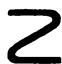
\includegraphics[keepaspectratio]{images/part001_36e9f8fa.jpg}}

\begin{enumerate}
\def\labelenumi{\arabic{enumi})}
\setcounter{enumi}{1}
\item
  Suppose that E is a quasi-Galois extension of K and F a quasi-Galois extension of E; it is not always the case that F is quasi-Galois over K (V, p.~153, Ex. 1). The reason is the following: let u be a K-automorphism of \(\Omega\) ; we have \(u(E) = E\) , but if f is the minimal polynomial over E of an element x of F, it is not necessarily invariant under u; therefore \(u(x)\) is not necessarily conjugate to x over E, and so need not necessarily belong to F. In that case F and \(u(F)\) are two distinct quasi-Galois extensions of E which are K-isomorphic but not E-isomorphic.
\item
  Let E be an algebraic extension of K and x, y two elements of E. If there exists a K-automorphism of E which maps x to y then x and y have the same minimal polynomial over K and so are conjugate over K by Prop. 2 (V, p.~52). The converse holds if E is quasi-Galois, because every K-automorphism of \(\Omega\) induces a K-automorphism of E. The hypothesis that E be quasi-Galois is not superfluous as the following example shows: let K = Q and \(\Omega\) the field of all algebraic numbers; put \(E = \Omega \cap R\) . It may be shown (V, p.~153, Ex. 2) that every automorphism of E is the identity mapping and that \(\sqrt{2}\) and \(-\sqrt{2}\) are elements of E conjugate over Q.
\end{enumerate}

\subsection{The quasi-Galois extension generated by a set}

PROPOSITION 4. --- Let \((\mathbf{N}_i)_{i\in I}\) be a family of quasi-Galois extensions of K contained in \(\Omega\) . Let \(\mathbf{N} = \bigcap_{i\in I}\mathbf{N}_i\) and \(\mathbf{M} = \mathbf{K}\left(\bigcup_{i\in I}\mathbf{N}_i\right)\) ; then the extensions N and M

of K are quasi-Galois.

Let \(u\) be a K-automorphism of \(\Omega\) . We have \(u(\mathbf{N}_i) = \mathbf{N}_i\) for all \(i \in I\) , hence we obtain the equalities \(u(\mathbf{N}) = \mathbf{N}\) and \(u(\mathbf{M}) = \mathbf{M}\) ; now the proposition follows from Cor. 1 (V, p.~54).

Let A be a set of elements of \(\Omega\) , and let B be the set of elements of \(\Omega\) which are conjugates of elements of A; expressed differently, if G is the group of K-automorphisms of \(\Omega\) , we have \(\mathbf{B} = \bigcup_{u \in G} u(\mathbf{A})\) . For each \(u \in G\) we have

\(u(B) = B\) whence \(u(K(B)) = K(B)\) . Therefore \(K(B)\) is a quasi-Galois extension of K containing A and it is immediate that every quasi-Galois extension N of K containing A contains B, hence \(K(B)\) . We shall say that \(K(B)\) is the quasi-Galois extension generated by A. This definition applies in particular when A is an extension of K.

The next proposition follows directly from the preceding remarks.

PROPOSITION 5. --- Let E be an extension of K contained in Ω and N the quasi-Galois extension generated by E. If A is a subset of Ω such that E = K(A) then N = K(B), where B is the set of elements of Ω which are conjugate to an element of A.

COROLLARY 1. --- If E is an extension of finite degree of K, then the quasi-Galois extension N of K generated by E is of finite degree over K.

For we have \(E = K(A)\) where A is finite, hence the set B of conjugates of elements of A is finite, whence the corollary follows by Th. 2 (V, p.~18).

COROLLARY 2. --- Every quasi-Galois extension N of K is the union of quasi-Galois subextensions of N of finite degree over K.

Let \(x \in \mathbb{N}\) and let \(\mathbf{N}_x\) be the quasi-Galois extension of \(\mathbf{K}\) generated by \(\{x\}\) . Since \(\mathbf{K}(x)\) is of finite degree over \(\mathbf{K}\) , the same is true of \(\mathbf{N}_x\) (Cor. 1) and we have \(x \in \mathbf{N}_x\) .

\section{GALOIS EXTENSIONS}

Throughout this paragraph K denotes a field.

\subsection{Definition of Galois extensions}

THEOREM 1. --- Let N be an algebraic extension of K and \(\Gamma\) the group of K-automorphisms of N. Then the following assertions are equivalent:

\begin{enumerate}
\def\labelenumi{\alph{enumi})}
\item
  Every element of \(\mathbf{N}\) invariant under \(\Gamma\) belongs to the image of \(\mathbf{K}\) in \(\mathbf{N}\) .
\item
  N is a separable quasi-Galois extension of K.
\item
  For each \(x \in \mathbf{N}\) the minimal polynomial of \(x\) over \(\mathbf{K}\) splits in \(\mathbf{N}[\mathbf{X}]\) into a product of distinct polynomials of degree 1.
\end{enumerate}

The equivalence of b) and c) follows from the Cor. of Prop. 6 (V, p.~40) and the definition of quasi-Galois extension (V, p.~53, Def. 2). Let us identify K with its canonical image in N.

\(a) \Rightarrow c)\) : Suppose that K is the field of invariants of \(\Gamma\) . Let \(x \in \mathbf{N}\) , with minimal polynomial \(f\) over K and let A be the set of all roots of \(f\) in N. Put

\[
g (\mathbf {X}) = \prod_ {y \in \mathsf {A}} (\mathbf {X} - y).
\]

Every automorphism \(\sigma \in \Gamma\) induces a permutation of \(\mathbf{A}\) , and hence leaves invariant the coefficients of the polynomial \(g \in \mathbf{N}[\mathbf{X}]\) . We thus have \(g \in \mathbf{K}[\mathbf{X}]\) and since \(g(x) = 0\) , the polynomial \(g\) is a multiple of \(f\) in \(\mathbf{K}[\mathbf{X}]\) (V, p.~16, Th. 1). Further, \(f\) and \(g\) are monic and \(g\) divides \(f\) (IV, p.~16, Prop. 5); thus we have \(f = g\) , which means that the minimal polynomial \(f\) of \(x\) over \(\mathbf{K}\) is a product in \(\mathbf{N}[\mathbf{X}]\) of distinct polynomials of degree 1.

\(c) \Rightarrow a)\) : let \(x\) be an element of \(\mathbf{N}\) not belonging to \(\mathbf{K}\) . Denote by \(\Omega\) an algebraic closure of \(\mathbf{K}\) containing \(\mathbf{N}\) as subextension (V, p.~23, Th. 2). Let \(f\) be the minimal polynomial of \(x\) over \(\mathbf{K}\) , which is of degree \(\geqslant 2\) by hypothesis and let \(\mathbf{A}\) be the set of roots of \(f(\mathbf{X})\) in \(\mathbf{N}\) . If condition \(c)\) holds, we have \(f(\mathbf{X}) = \prod_{y \in \mathbf{A}} (\mathbf{X} - y)\) and so

(V, p.~53, Cor. 1) A is the set of conjugates of \(x\) in \(\Omega\) . Since \(f\) has degree \(\geqslant 2\) , there exists in A an element \(y \neq x\) , hence a K-automorphism \(u\) of \(\Omega\) such that \(u(x) = y\) . Now under the hypothesis \(c\) ), the extension N of K is quasi-Galois, hence \(u(N) = N\) (V, p.~54, Cor. 1); it follows that \(u\) induces a K-automorphism \(\sigma\) of N such that \(\sigma(x) = y \neq x\) , so K is the field of invariants of \(\Gamma\) .

DEFINITION 1. --- An extension N of K is said to be Galois if it is algebraic and satisfies the equivalent conditions a), b), c) of Th. 1.

Let N be a field, \(\Gamma\) a group of automorphisms of N and \(N_{0}\) the field of invariants of \(\Gamma\) . When N is algebraic over \(N_{0}\) it is a Galois extension of \(N_{0}\) . This need not always be so: for example, suppose that K is infinite and take N to be the field of rational fractions \(\mathrm{K}(\mathrm{X})\) ; for each \(a \in K\) let \(\sigma_{a}\) be the automorphism of \(\mathrm{K}(\mathrm{X})\) which maps \(f(\mathrm{X})\) to \(f(\mathrm{X} + a)\) . The set of all \(\sigma_{a}\) is a group of automorphisms of \(\mathrm{K}(\mathrm{X})\) whose field of invariants is easily seen to be K; however \(\mathrm{K}(\mathrm{X})\) is not algebraic over K.

Let \(\Omega\) be an algebraic closure of K, let A denote a set of elements of \(\Omega\) separable over K and B the set of conjugates over K of elements of A. Then B consists of elements that are algebraic and separable over K. Therefore (V, p.~39, Prop. 6 and p.~56, Prop. 5) the field K(B) is a separable quasi-Galois extension of K; in other words, the quasi-Galois extension generated by A (V, p.~55) is a Galois extension of K; we shall also say that it is the Galois extension of K generated by the subset A of \(\Omega\) .

In particular, the splitting field in \(\Omega\) of a family of separable polynomials over K, a separable closure of K, are Galois extensions of K.

PROPOSITION 1. --- Let N be an extension of K and \((\mathbf{N}_{i})_{i\in I}\) a non-empty family of subextensions of N. We put \(E=\bigcap_{i\in I}N_{i}\) and \(F=K\left(\bigcup_{i\in I}N_{i}\right)\) . If all the extensions

\(N_{i}\) are Galois over K then the same is true of E and F.

In the first place E is algebraic and separable over K (V, p.~36, Prop. 1) and the same holds for F (V, p.~41, Prop. 8). Moreover, E and F are quasi-Galois over K by Prop. 4 (V, p.~55).

PROPOSITION 2. --- Let N be a Galois extension of K and E a subextension of N, of finite degree over K. There exists a subextension F of N containing E, Galois and of finite degree over K.

Since N is quasi-Galois over K, Cor. 1 of V, p.~56 proves the existence of a quasi-Galois subextension F of N containing E and of finite degree over K. Since N is separable over K, the same holds for F (V, p.~36, Prop. 1), hence F is Galois over K.

Prop. 2 implies the following result: let \(\Omega\) be an algebraic closure of K and \(E_1, \ldots, E_n\) separable algebraic extensions of finite degree over K, contained in \(\Omega\) . Then there exists a Galois extension N of K, of finite degree, contained in \(\Omega\) and containing \(E_1, \ldots, E_n\) .

\subsection{The Galois group}

DEFINITION 2. --- Let N be a Galois extension of the field K. The group of all K-automorphisms of N will be called the Galois group of N over K and denoted by Gal(N/K).

Let N be a finite Galois extension of K. Then N is a finite separable and quasi-Galois extension of K. Therefore (V, p.~32, Prop. 4 and V, p.~54, Prop. 3), the order of Gal(N/K) is equal to {[}N : K{]}. We shall prove later that if N is a Galois extension of K such that Gal(N/K) is finite, then N is of finite degree over K (V, p.~66, Th. 3).

Let \(\Omega\) be an algebraically closed extension of K and let A be the set of roots in \(\Omega\) of a separable polynomial \(f \in \mathbf{K}[\mathbf{X}]\) . Then the field \(\mathbf{N} = \mathbf{K}(\mathbf{A})\) is a Galois extension of K. It is clear that every K-automorphism of N leaves A stable, and since A generates N over K, the mapping \(\sigma \mapsto \sigma | \mathbf{A}\) is an isomorphism of \(\operatorname{Gal}(\mathbf{N} / \mathbf{K})\) onto a subgroup \(\Gamma\) of the symmetric group \(\mathfrak{S}_{\mathbf{A}}\) of the set A, which will be called the Galois group of the polynomial \(f\) . From Remark 3 (V, p.~55) it follows that if \(x\) and \(y\) belong to A, the following properties are equivalent:

\begin{enumerate}
\def\labelenumi{\alph{enumi})}
\item
  \(x\) and \(y\) are conjugate over \(\mathbf{K}\) ,
\item
  \(x\) and \(y\) belong to the same orbit under \(\Gamma\) ,
\item
  \(x\) and \(y\) are roots of the same irreducible factor of \(f\) .
\end{enumerate}

In particular \(f\) is irreducible if and only if \(\mathbf{A}\) is non-empty and \(\Gamma\) operates transitively on \(\mathbf{A}\) .

Examples. --- 1) Suppose that the characteristic of K is different from 2 and let N be a quadratic extension of K. If \(x \in \mathbf{N} - \mathbf{K}\) , then we have \(\mathbf{N} = \mathbf{K}(x)\) and the minimal polynomial of \(x\) over K is of the form \(f(\mathbf{X}) = \mathbf{X}^2 - a\mathbf{X} + b\) , with \(a, b \in \mathbf{K}\) . We thus have \(f(\mathbf{X}) = (\mathbf{X} - x)(\mathbf{X} - y)\) where \(y = a - x\) , so \(y\) is conjugate to \(x\) ; since \(f(\mathbf{X})\) is separable, the extension N is Galois. The group \(\operatorname{Gal}(\mathbf{N}/\mathbf{K})\) has two elements which induce the two permutations of the set \(\{x, y\}\) .

2) Let \(f = \mathbf{X}^3 + \mathbf{X}^2 - 2\mathbf{X} - 1 \in \mathbf{Q}[\mathbf{X}]\) . The polynomial \(f\) is irreducible, for if not, then it would have a root \(x \in \mathbf{Q}\) ; on writing \(x = a / b\) with \(a, b \in \mathbf{Z}\) , \(a\) and \(b\) relatively prime, we should find \(a(a^2 + ab - 2b^2) = b^3\) and \(a^3 = b(b^2 + 2ab - a^2)\) ; but this implies that \(a\) divides \(b\) and \(b\) divides \(a\) , hence \(x = \pm 1\) , which is impossible. Put \(\xi = e^{2\pi i / 7} \in \mathbf{C}\) ; then the polynomial \(f\) has the roots \(\alpha = \xi + \xi^{-1}, \beta = \xi^2 + \xi^{-2}, \gamma = \xi^3 + \xi^{-3}\) . We have \(\beta = \alpha^2 - 2\) and \(\gamma = \alpha^3 - 3\alpha\) , hence the extension \(\mathbf{Q}(\alpha)\) is Galois over \(\mathbf{Q}\) . The Galois group of \(\mathbf{Q}(\alpha)\) over \(\mathbf{Q}\) is cyclic of order 3 and is generated by an element \(\sigma\) such that \(\sigma(\alpha) = \beta, \sigma(\beta) = \gamma, \sigma(\gamma) = \alpha.\)

\begin{enumerate}
\def\labelenumi{\arabic{enumi})}
\setcounter{enumi}{2}
\item
  Suppose that K = Q and take \(f = X^{3} - 2\) . Using the decomposition of integers into products of prime factors (I, p.~51), we easily see that 2 is not the cube of an element of Q. Hence the polynomial f is irreducible, for if not, it would have a root in Q. Let \(A = \{x_{1}, x_{2}, x_{3}\}\) be the set of roots of f in \(\Omega\) and \(\Gamma\) the Galois group of f.~It acts transitively on A; its order is therefore divisible by three. On the other hand, the quotient \(j = \frac{x_{2}}{x_{1}}\) is different from 1 and we have \(j^{3} = 1\) . Hence j satisfies the relation \(j^{2} + j + 1 = 0\) ; now the polynomial \(T^{2} + T + 1 = \left(T + \frac{1}{2}\right)^{2} + \frac{3}{4}\) has no roots in Q, which shows (Example 1) that \([Q(j): Q] = 2\) . Thus \([N: Q]\) is divisible by 2, and it follows that the order of \(\Gamma\) is divisible by 6. Since \(\Gamma\) is contained in the group \(S_{A}\) of order 6, we have \(\Gamma = S_{A}\) .
\item
  Suppose that K is of characteristic \(p \neq 0\) and let \(\mathrm{K}(\mathrm{T})\) be the field of rational fractions and \(U = T^{p} - T\) . Put \(E = K[U]\) and \(F = K[T]\) , then the polynomial \(f(X) = X^{p} - X - U\) of \(E[X]\) has the roots \(T, T + 1, \ldots, T + p - 1\) in F. Let \(\sigma\) be the K-automorphism of F such that \(\sigma(T) = T + 1\) . We have \(\sigma^{i}(T) = T + i\) and \(\sigma(U) = U\) . The group \(G = \{1, \sigma, \ldots, \sigma^{p-1}\}\) is cyclic of order p, and its field of invariants contains E; since \([F: E] \leqslant p\) , Dedekind's theorem (V, p.~27, Cor. 2) implies that E is the field of invariants of G and \([F: E] = p\) . The polynomial f is thus irreducible in \(E[X]\) ; the extension F of E is Galois, its Galois group G is cyclic of order p, and the group \(\Gamma\) is the group of cyclic permutations of T, \(T + 1, \ldots, T + p - 1\) .
\end{enumerate}

For a generalization of this example see V, p.~93, Example 2.

\begin{enumerate}
\def\labelenumi{\arabic{enumi})}
\setcounter{enumi}{4}
\tightlist
\item
  Let \(\mathbf{F} = \mathbf{K}(\mathbf{X}_1, \ldots, \mathbf{X}_n)\) be the field of rational fractions in \(n\) indeterminates \(\mathbf{X}_1, \ldots, \mathbf{X}_n\) with coefficients in \(\mathbf{K}\) . Put
\end{enumerate}

\[
s _ {k} = \sum_ {1 \leqslant i _ {1} <   \dots <   i _ {k} \leqslant n} X _ {i _ {1}} \dots X _ {i _ {k}}
\]

for \(1 \leqslant k \leqslant n\) and \(\mathrm{E} = \mathrm{K}(s_1, \ldots, s_n)\) ; we denote by \(f(\mathrm{T})\) the polynomial

\[
\mathrm{T} ^ {n} - s _ {1} \mathrm{T} ^ {n - 1} + \dots + (- 1) ^ {n} s _ {n}.
\]

We have \(f(\mathrm{T}) = \prod_{i=1}^{n} (\mathrm{T} - \mathrm{X}_i)\) , so that \(\mathbf{F}\) is a splitting field of the separable polynomial \(f(\mathrm{T}) \in \mathrm{E}[\mathrm{T}]\) . Further, for every permutation \(\sigma \in \mathfrak{S}_n\) there exists a unique \(\mathbf{K}\) -automorphism \(h_\sigma\) of \(\mathbf{F}\) such that \(h_\sigma(\mathrm{X}_i) = \mathrm{X}_{\sigma(i)}\) for \(1 \leqslant i \leqslant n\) ; we have \(h_\sigma(s_k) = s_k\) for \(1 \leqslant k \leqslant n\) , hence \(h_\sigma\) is an E-automorphism of \(\mathbf{F}\) . In other words, \(\mathbf{F}\) is a Galois extension of \(\mathbf{E}\) and the restriction to the set of roots \(\{\mathbf{X}_1, ..., \mathbf{X}_n\}\) of \(f(\mathrm{T})\) defines an isomorphism of \(\operatorname{Gal}(\mathrm{F}/\mathrm{E})\) onto the group \(\mathfrak{S}_n\) . In particular, \(\mathbf{E}\) consists of rational fractions \(f\) such that

\[
f \left(\mathrm{X} _ {\sigma (1)}, \dots , \mathrm{X} _ {\sigma (n)}\right) = f \left(\mathrm{X} _ {1}, \dots , \mathrm{X} _ {n}\right)
\]

for every \(\sigma \in \mathfrak{S}_n\) (cf.~IV, p.~67, Cor.).

\begin{enumerate}
\def\labelenumi{\arabic{enumi})}
\setcounter{enumi}{5}
\tightlist
\item
  Suppose that \(f\) is monic of degree \(> 0\) and \(K\) is of characteristic \(\neq 2\) . Define on \(A\) a total ordering, denoted by \(\leqslant\) , and put \(\delta(f) = \prod_{\alpha < \beta} (\beta - \alpha)\) ,
\end{enumerate}

\((\alpha, \beta) \in \mathbf{A} \times \mathbf{A}\) , and for each \(\sigma \in \mathfrak{S}_{\mathbf{A}}\) put \(\delta_{\sigma}(f) = \prod_{\alpha < \beta} (\sigma(\beta) - \sigma(\alpha))\) . We have

\(\delta_{\sigma}(f) = \varepsilon(\sigma)\ \delta(f)\) , where \(\varepsilon(\sigma)\) is the signature of \(\sigma\) (I, p.~64) and \(\delta(f) \neq 0\) . For every \(\tau \in \operatorname{Gal}(\mathbf{N}/\mathbf{K})\) we have \(\tau(\delta(f)) = \delta_{\tau|_{\mathbf{A}}}(f)\) . Hence \(\Gamma\) is contained in the alternating group \(\mathfrak{A}_{\mathbf{A}}\) if and only if \(\delta(f) \in \mathbf{K}\) . Moreover \(\delta(f)^2 = \prod_{\alpha < \beta} (\beta - \alpha)^2 =\)

\(d(f)\) is the discriminant of the polynomial \(f\) (IV, p.~81) . Hence \(\Gamma \subset \mathfrak{A}_{\mathbf{A}}\) if and only if \(d(f)\) is the square of an element of \(\mathbf{K}\) . Thus in Example 2 we have \(d(f) = 49 = 7^2\) and in Example 3, \(d(f) = -108\) (IV, p.~85).

Let N be a Galois extension of K and let L be a subextension of N which is Galois over K. Every K-automorphism \(\sigma\) of N induces a K-automorphism \(\sigma_{L}\) of L (V, p.~55, Remark 1). Therefore the mapping \(\sigma \mapsto \sigma_{L}\) is a homomorphism of \(\operatorname{Gal}(N/K)\) into \(\operatorname{Gal}(L/K)\) , called the restriction homomorphism.

PROPOSITION 3. --- The restriction homomorphism of Gal(N/K) into Gal(L/K) is surjective.

More generally, consider two subextensions L and L' of N, and a K-isomorphism u of L onto L'. Choose an algebraic closure \(\Omega\) of K containing N as subextension (V, p.~23, Th. 2). There exists a K-automorphism v of \(\Omega\) which coincides with u on L (V, p.~52, Prop. 1), and since N is a quasi-Galois extension of K, v induces a K-automorphism \(\sigma\) of N (V, p.~55, Remark 1). In other words, the element \(\sigma\) of Gal(N/K) coincides with u on L.

\subsection{Topology of the Galois group}

Let N be a Galois extension of K and \(\Gamma\) the Galois group of N over K. We equip N with the discrete topology, the set \(N^{N}\) of all mappings of N into itself with the product topology of the discrete topology of the factors (« topology of simple convergence in N ») and the group \(\Gamma\) with the topology induced from \(N^{N}\) .

Let \(\Lambda\) be the set of all subextensions of \(\mathbf{N}\) of finite degree over \(\mathbf{K}\) . For \(\sigma \in \Gamma\) and \(\mathrm{E} \in \Lambda\) we shall write \(\mathrm{U}_{\mathrm{E}}(\sigma)\) for the set of elements \(\tau\) of \(\Gamma\) which have the same restriction as \(\sigma\) to \(\mathrm{E}\) . If \(\mathrm{E} = \mathrm{K}(x_1, \ldots, x_n)\) , the set \(\mathrm{U}_{\mathrm{E}}(\sigma)\) consists of the elements \(\tau \in \Gamma\) such that \(\tau(x_1) = \sigma(x_1), \ldots, \tau(x_n) = \sigma(x_n)\) . It follows that the family \((\mathrm{U}_{\mathrm{E}}(\sigma))_{\mathrm{E} \in \Lambda}\) is a base of the filter of neighbourhoods of \(\sigma\) in \(\Gamma\) .

When N is of finite degree over K, we have \(N \in \Lambda\) and \(U_{N}(\sigma) = \{\sigma\}\) , hence the topology of \(\operatorname{Gal}(N/K)\) is discrete; we recall (V, p.~58), that the group \(\operatorname{Gal}(N/K)\) is finite in this case.

This description of the topology of \(\operatorname{Gal}(\mathbf{N}/\mathbf{K})\) shows that the restriction homomorphism of \(\operatorname{Gal}(\mathbf{N}/\mathbf{K})\) onto \(\operatorname{Gal}(\mathbf{L}/\mathbf{K})\) is continuous for every subextension L of N which is Galois over N.

Let A be a subset of \(\Gamma\) . To say that A is open means that for each \(\sigma\in A\) there exists E in \(\Lambda\) such that the set \(U_{E}(\sigma)\) is contained in A. The closure \(\bar{A}\) of A consists of all \(\sigma\in\Gamma\) such that for any \(E\in\Lambda\) there exists \(\tau\in A\) having the same restriction to E as \(\sigma\) ; the field of invariants of \(\bar{A}\) is the same as that of A.

Let \(\varepsilon\) be the neutral element of \(\Gamma\) and let \(\Lambda'\) be the set of subextensions of \(N\) which are Galois and of finite degree over \(K\) . By Prop. 2 (V, p.~57) the set \(\Lambda'\) is cofinal in \(\Lambda\) and the family \((U_E(\varepsilon))_{E \in \Lambda'}\) is thus a base of the filter of neighbourhoods of \(\varepsilon\) in \(\Gamma\) . Further, for \(E \in \Lambda'\) the set \(U_E(\varepsilon)\) is the kernel of the restriction homomorphism of \(\operatorname{Gal}(N/K) = \Gamma\) into \(\operatorname{Gal}(E/K)\) . Since \(\operatorname{Gal}(E/K)\) is finite, it follows that \(U_E(\varepsilon)\) is an open and closed subgroup, normal and of finite index in \(\Gamma\) .

Clearly we have \(\mathrm{U}_{\mathrm{E}}(\sigma)=\sigma\mathrm{U}_{\mathrm{E}}(\varepsilon)=\mathrm{U}_{\mathrm{E}}(\varepsilon)\sigma\) for \(\sigma\in\Gamma\) and \(E\in\Lambda'\) . Since \(\mathrm{U}_{\mathrm{E}}(\varepsilon)\) is a normal subgroup of \(\Gamma\) for all \(E\in\Lambda'\) and the family \((\mathrm{U}_{\mathrm{E}}(\varepsilon))_{E\in\Lambda'}\) is a base of neighbourhoods at \(\varepsilon\) , the topology of \(\Gamma\) is compatible with the group structure (Gen.~Top., III, p.~223). In other words, the mapping \((\sigma,\tau)\mapsto\sigma\tau^{-1}\) of \(\Gamma\times\Gamma\) into \(\Gamma\) is continuous.

PROPOSITION 4. --- Let N be a Galois extension of K. Then the Galois group \(\Gamma = \operatorname{Gal}(\mathbf{N}/\mathbf{K})\) is compact and totally disconnected.

Every element \(\sigma\) of \(\Gamma\) has a base of neighbourhoods consisting of the open and closed sets \(U_{E}(\sigma)\) , hence \(\Gamma\) is totally disconnected (Gen.~Top., I, p.~111). We have \(\{\sigma\} = \bigcap_{E \in \Lambda} U_{E}(\sigma)\) , hence \(\Gamma\) is separated. For each \(x \in \mathbb{N}\) the set of conjugates

\(\sigma(x)\) of \(x\) , as \(\sigma\) ranges over \(\Gamma\) , is finite because \(x\) is algebraic over K (V, p.~53, Cor. 1); hence all the projections of \(\Gamma\) on the factor spaces of \(\mathbf{N}^{\mathbb{N}}\) are finite sets, and this shows \(\Gamma\) to be relatively compact in \(\mathbf{N}^{\mathbb{N}}\) (Gen.~Top., I, p.~88). It remains to show that \(\Gamma\) is closed in \(\mathbf{N}^{\mathbb{N}}\) . Now if \(u\) is in the closure of \(\Gamma\) in \(\mathbf{N}^{\mathbb{N}}\) , then for each pair of points \((x,y)\) of N there exists \(\sigma \in \Gamma\) with \(u(x) = \sigma(x)\) , \(u(y) = \sigma(y)\) , \(u(x + y) = \sigma(x + y)\) , \(u(xy) = \sigma(xy)\) , whence \(u(x + y) = u(x) + u(y)\) and \(u(xy) = u(x)u(y)\) . By the same reasoning we have \(u(x) = x\) for all \(x \in \mathbf{K}\) , hence \(u\) is a K-homomorphism of N into N; since N is algebraic over K, \(u\) is a K-automorphism of N (V, p.~52, Prop. 1), hence \(u \in \Gamma\) .

Let N be a Galois extension of K and \((\mathbf{N}_{i})_{i\in I}\) an increasing directed family of subextensions of N. Suppose that \(N_{i}\) is Galois over K for all \(i\in I\) and that \(N=\bigcup_{i\in I}N_{i}\) . For each \(i\in I\) denote by \(\Gamma_{i}\) the Galois group of \(N_{i}\) over K; for

\(i \leqslant j\) in I we have \(N_i \subset N_j\) and the restriction homomorphism \(\varphi_{ij}\) of \(\Gamma_j\) into \(\Gamma_i\) is defined. It is continuous and so the family \((\Gamma_i, \varphi_{ij})\) is an inverse system of topological groups. Further, for each \(i \in I\) denote by \(\lambda_i\) the restriction homomorphism of \(\text{Gal}(N/K)\) into \(\text{Gal}(N_i/K) = \Gamma_i\) ; it is continuous and we have \(\lambda_i = \varphi_{ij} \circ \lambda_j\) for \(i \leqslant j\) , hence the family \((\lambda_i)_{i \in I}\) defines a continuous homomorphism \(\lambda\) of \(\text{Gal}(N/K)\) into \(\varprojlim \Gamma_i\) .

PROPOSITION 5. --- The homomorphism \(\lambda\) of \(\operatorname{Gal}(\mathbf{N}/\mathbf{K})\) into \(\varprojlim \operatorname{Gal}(\mathbf{N}_i/\mathbf{K})\) is an isomorphism of topological groups.

Since \(\operatorname{Gal}(\mathbf{N}/\mathbf{K})\) is compact, \(\lambda\) continuous and the group \(\varprojlim \operatorname{Gal}(\mathbf{N}_i/\mathbf{K})\) separated, it suffices to show that \(\lambda\) is bijective (Gen.~Top., I, p.~87, Cor. 2). Let \(u = (u_i)_{i \in I}\) be an element of \(\varprojlim \operatorname{Gal}(\mathbf{N}_i/\mathbf{K})\) ; for each \(i \in I\) , \(u_i\) is a K-automorphism of \(\mathbf{N}_i\) and \(u_i\) is the restriction of \(u_j\) to \(\mathbf{N}_i\) for \(i \leqslant j\) . Since \(\mathbf{N} = \bigcup_{i \in I} \mathbf{N}_i\) there exists a unique element \(\sigma\) of \(\operatorname{Gal}(\mathbf{N}/\mathbf{K})\) which coincides with

\(u_{i}\) on \(\mathbf{N}_i\) for all \(i\in \mathbf{I}\) . Thus \(\sigma\) is the unique element of \(\operatorname {Gal}(\mathbf{N} / \mathbf{K})\) such that \(\lambda (\sigma) = u\) , hence \(\lambda\) is bijective.

This applies in particular when we take for the family \((\mathbf{N}_{i})\) the family of all finite Galois subextensions of N; then each group \(\operatorname{Gal}(\mathbf{N}_{i}/\mathbf{K})\) is discrete and finite. The topological group \(\operatorname{Gal}(\mathbf{N}/\mathbf{K})\) is thus isomorphic to a directed inverse limit of finite groups, equipped with the discrete topology; this is sometimes called a profinite topological group.

\subsection{Galois descent}

In this No.~we denote by N a field, \(\Gamma\) a group of automorphisms of N, \(\varepsilon\) the neutral element of \(\Gamma\) and K the field of invariants of \(\Gamma\) .

Let \(\mathbf{V}\) be a vector space over \(\mathbf{N}\) . We recall (II, p.~317) that a K-structure on \(\mathbf{V}\) is a vector sub-K-space \(\mathbf{V}_0\) of \(\mathbf{V}\) such that the K-linear mapping \(\varphi: \mathbf{N} \otimes_{\mathbf{K}} \mathbf{V}_0 \to \mathbf{V}\) which maps \(\lambda \otimes x\) to \(\lambda x\) is bijective. Let \(\mathbf{V}_0\) be such a K-structure; for each \(\sigma \in \Gamma\) we put \(u_\sigma = \varphi \circ (\sigma \otimes \mathrm{Id}_{\mathbf{V}_0}) \circ \varphi^{-1}\) ; then we have \(u_\sigma \left( \sum_{i \in I} \lambda_i e_i \right) = \sum_{i \in I} \sigma(\lambda_i) e_i\)

for every family of elements \(\lambda_{i}\) of \(\mathbf{N}\) and \(e_i\) of \(\mathbf{V}_0\) whence we obtain the relations

\[
u _ {\sigma} (x + y) = u _ {\sigma} (x) + u _ {\sigma} (y)\tag{1}
\]

\[
u _ {\sigma} (\lambda x) = \sigma (\lambda) u _ {\sigma} (x)\tag{2}
\]

\[
u _ {\sigma} \circ u _ {\tau} = u _ {\sigma \tau}\tag{3}
\]

\[
u _ {\varepsilon} = \operatorname{Id} _ {\mathrm{V}}\tag{4}
\]

for \(\sigma, \tau\) in \(\Gamma\) , \(x, y\) in \(\mathbf{V}\) and \(\lambda\) in \(\mathbf{N}\) .

PROPOSITION 6. --- a) Let V be a vector space over N with a K-structure. For a vector \(x \in V\) to be rational over K it is necessary and sufficient that \(u_{\sigma}(x) = x\) for all \(\sigma \in \Gamma\) . For a vector sub-N-space W of V to be rational over K it is necessary and sufficient that \(u_{\sigma}(W) \subset W\) for all \(\sigma \in \Gamma\) .

\begin{enumerate}
\def\labelenumi{\alph{enumi})}
\setcounter{enumi}{1}
\tightlist
\item
  Let \(V_{1}\) and \(V_{2}\) be two vector spaces over N, each with a K-structure. For a linear mapping of \(V_{1}\) into \(V_{2}\) to be rational over K it is necessary and sufficient that \(f(u_{\sigma}(x)) = u_{\sigma}(f(x))\) for all \(\sigma \in \Gamma\) and all \(x \in V_{1}\) .
\end{enumerate}

It is clear that K is the set of \(x \in N\) such that \(\sigma(xy) = x\sigma(y)\) for all \(\sigma \in \Gamma\) and all \(y \in N\) . The proposition therefore follows from Th. 1 (II, p.~324).

COROLLARY. --- Let \(V_{0}\) be a vector space over K and let W be a vector sub-N-space of \(N \otimes_{K} V_{0}\) . Suppose that W is stable under the mappings \(\sigma \otimes Id_{V_{0}}\) for all \(\sigma \in \Gamma\) . Let \(W_{0}\) be the set of \(x \in V_{0}\) such that \(1 \otimes x \in W\) ; then \(W_{0}\) is the unique vector sub-K-space of \(V_{0}\) such that \(W = N \otimes_{K} W_{0}\) .

It suffices to remark that the set of elements of the form \(1 \otimes x\) ( \(x \in \mathbf{V}_0\) ) is a K-structure on \(\mathbf{N} \otimes_{\mathbf{K}} \mathbf{V}_0\) for which we have \(u_\sigma = \sigma \otimes \mathrm{Id}_{\mathbf{V}_0}\) for \(\sigma \in \Gamma\) .

PROPOSITION 7. --- Let V be a vector space over N, \((u_{\sigma})_{\sigma \in \Gamma}\) a family of mappings of V into itself satisfying (1) to (4) and \(V_{0}\) the set of \(x \in V\) such that \(u_{\sigma}(x) = x\) for all \(\sigma \in \Gamma\) .

\begin{enumerate}
\def\labelenumi{\alph{enumi})}
\item
  \(\mathbf{V}_0\) is a vector sub-K-space of \(\mathbf{V}\) and the K-linear mapping \(\varphi\) of \(\mathbf{N} \otimes_{\mathbf{K}} \mathbf{V}_0\) into \(\mathbf{V}\) which maps \(\lambda \otimes x\) to \(\lambda x\) is injective.
\item
  If \(\Gamma\) is finite, then \(\varphi\) is bijective and \(\mathbf{V}_0\) is a K-structure on \(\mathbf{V}\) .
\end{enumerate}

It is clear that \(\mathbf{V}_0\) is a vector sub-K-space of \(\mathbf{V}\) .

The formula \(u_{\sigma} \circ \varphi = \varphi \circ (\sigma \otimes \operatorname{Id}_{\mathbf{V}_{0}})\) shows that the kernel W of \(\varphi\) is stable under the mappings \(\sigma \otimes \operatorname{Id}_{\mathbf{V}_{0}}\) ; by the Cor. to Prop. 6 there exists therefore a subspace \(W_{0}\) of \(V_{0}\) such that \(W = N \otimes_{K} W_{0}\) . If x belongs to \(W_{0}\) we then have \(x = \varphi(1 \otimes x) = 0\) , hence \(W_{0} = 0\) and so W = 0. This proves a).

Suppose now that \(\Gamma\) is finite; we have to show that \(\varphi\) is surjective, or equivalently that \(V_0\) generates the vector N-space V. Thus let \(f\) be an N-linear form on V whose restriction to \(V_0\) is zero. Let \(x \in V\) ; for every \(\lambda \in N\) the element \(y_\lambda = \sum_{\sigma \in \Gamma} u_\sigma(\lambda x)\) of V clearly belongs to \(V_0\) , whence \(f(y_\lambda) = 0\) , that is,

\(\sum_{\sigma \in \Gamma}f(u_{\sigma}(x))\sigma (\lambda) = 0\) . By Dedekind's theorem (V, p.~27, Cor. 2) we thus have

\(f(u_{\sigma}(x)) = 0\) for each \(\sigma \in \Gamma\) ; in particular, taking \(\sigma = \varepsilon\) we find \(f(x) = 0\) , which means that \(f = 0\) . This proves \(b\) ).

Let \(\mathbf{M}\) be a vector space over \(\mathbf{N}\) ; for each \(\sigma \in \Gamma\) let \(\mathbf{M}^{\sigma}\) be the vector space over \(\mathbf{N}\) with the same underlying additive group as \(\mathbf{M}\) , with the external law \((\lambda, x) \mapsto \sigma(\lambda)x\) . Write \(\mathbf{V} = \prod_{\sigma \in \Gamma} \mathbf{M}^{\sigma}\) ; the underlying additive group of \(\mathbf{V}\) is that of

all mappings of \(\Gamma\) into \(\mathbf{M}\) , with the external law defined by

\[
(\lambda . h) (\sigma) = \sigma (\lambda) h (\sigma) \quad (\lambda \in \mathrm{N}, h \in \mathrm{V}, \sigma \in \Gamma).\tag{5}
\]

(The product \(\sigma(\lambda) h(\sigma)\) is calculated in the vector space M.) Further, we define on \(\mathbf{N} \otimes_{\mathbf{K}} \mathbf{M}\) a vector space structure over \(\mathbf{N}\) by the formula

\[
\lambda \left(\sum_ {i} \mu_ {i} \otimes x _ {i}\right) = \sum_ {i} \lambda \mu_ {i} \otimes x _ {i}.
\]

Finally we denote by \(\psi\) the K-linear mapping of \(\mathbf{N} \otimes_{\mathbf{K}} \mathbf{M}\) into \(\mathbf{V}\) characterized by the relation

\[
\psi (\lambda \otimes x) (\sigma) = \sigma (\lambda). x\tag{6}
\]

for \(\lambda \in \mathbf{N}\) , \(x \in \mathbf{M}\) and \(\sigma \in \Gamma\) . It is clear that \(\psi\) is N-linear.

PROPOSITION 8. --- The N-linear mapping \(\psi\) of \(\mathbf{N} \otimes_{\mathbf{K}} \mathbf{M}\) into \(\mathbf{V} = \prod_{\sigma \in \Gamma} \mathbf{M}^{\sigma}\) is

injective, and it is bijective if \(\Gamma\) is finite.

For every \(\sigma\in\Gamma\) we define a mapping \(u_{\sigma}\) of V into V by

\[
\left(u _ {\sigma} h\right) (\tau) = h (\tau \sigma)\tag{7}
\]

for \(h \in \mathbf{V}\) and \(\tau \in \Gamma\) . The verification of (1)-(4) is immediate. Denote by \(\mathbf{V}_0\) the set of \(h \in \mathbf{V}\) such that \(u_{\sigma}(h) = h\) for all \(\sigma \in \Gamma\) . For each \(x \in \mathbf{M}\) let \(\theta(x)\) be the constant mapping of \(\Gamma\) into \(\mathbf{M}\) with value \(x\) ; then \(\theta\) is a K-isomorphism of \(\mathbf{M}\) onto \(\mathbf{V}_0\) . If we define the homomorphism \(\varphi: \mathbf{N} \otimes_{\mathbf{K}} \mathbf{V}_0 \to \mathbf{V}\) as above, we have \(\psi = \varphi \circ (\mathrm{Id}_{\mathbf{N}} \otimes \theta)\) and now Prop. 8 follows from Prop. 7.

COROLLARY. --- Let \(\psi\) be the K-linear mapping of N \(\otimes_{K}\) N into the product vector space \(N^{\Gamma}\) such that \(\psi(x \otimes y) (\sigma) = \sigma(x)y\) for x, y in N and \(\sigma \in \Gamma\) . Then \(\psi\) is injective and it is bijective when \(\Gamma\) is finite.

This is the particular case \(\mathbf{M} = \mathbf{N}\) of Prop. 8.

Remarks. --- 1) Let F be an extension of K and N a subextension of F, and let \(\Gamma\) be a finite group of automorphisms of N, of which K is the field of invariants. Prop. 8 implies the existence of an isomorphism of K-algebras \(\theta: \mathbf{N} \otimes_{\mathbf{K}} \mathbf{F} \to \mathbf{F}^{\Gamma}\) characterized by \(\theta(x \otimes y)\) ( \(\sigma\) ) = \(\sigma(x)y\) for \(x \in \mathbf{N}\) , \(y \in \mathbf{F}\) and \(\sigma \in \Gamma\) .

\begin{enumerate}
\def\labelenumi{\arabic{enumi})}
\setcounter{enumi}{1}
\tightlist
\item
  The notation K, N and \(\Gamma\) has the same meaning as before. For each integer \(n \geqslant 1\) , let \(A_{n}\) be the tensor product of n K-algebras identical with N; let \(B_{n}\) be the set of mappings of \(\Gamma^{n-1}\) into N. By induction on n we can deduce from the Cor. of Prop. 8 the existence of an isomorphism \(\varphi_{n}: A_{n} \to B_{n}\) mapping \(x_{1} \otimes \ldots \otimes x_{n}\) to the function \((\sigma_{1}, \ldots, \sigma_{n-1}) \mapsto \sigma_{1}(x_{1}) \ldots \sigma_{n-1}(x_{n-1}) x_{n}\) .
\end{enumerate}

\subsection{Galois cohomology}

Let N be a field, \(\Gamma\) a finite group of automorphisms of N and K the field of invariants of \(\Gamma\) . For every integer \(n \geqslant 1\) we denote by \(\mathbf{GL}(n, \mathbf{N})\) the group of square matrices of order n with coefficients in N and non-zero determinant (II, p.~349). We let the group \(\Gamma\) operate on the group \(\mathbf{GL}(n, \mathbf{N})\) by the rule \(\sigma(A) = (\sigma(a_{ij}))\) for \(A = (a_{ij})\) .

PROPOSITION 9. --- Let \((U_{\sigma})_{\sigma \in \Gamma}\) be a family of elements of \(\mathbf{GL}(n, \mathbf{N})\) . For \(A\) to exist in \(\mathbf{GL}(n, \mathbf{N})\) such that \(U_{\sigma} = A^{-1} \cdot \sigma(A)\) for all \(\sigma \in \Gamma\) it is necessary and sufficient that \(U_{\sigma\tau} = U_{\sigma} \cdot \sigma(U_{\tau})\) for \(\sigma, \tau\) in \(\Gamma\) .

The condition is necessary: if \(U_{\sigma} = A^{-1} \cdot \sigma(A)\) , then we have

\[
U _ {\sigma} \cdot \sigma (U _ {\tau}) = A ^ {- 1} \cdot \sigma (A) \sigma (A ^ {- 1} \cdot \tau (A)) = A ^ {- 1} \sigma \tau (A) = U _ {\sigma \tau}.
\]

The condition is sufficient: we identify the elements of \(\mathbf{N}^n\) with matrices of \(n\) rows and one column with coefficients in \(\mathbf{N}\) . We let the groups \(\Gamma\) act on \(\mathbf{N}^n\) by

\[
\sigma (x) = \left(\sigma \left(x _ {i}\right)\right) _ {1 \leqslant i \leqslant n} \quad \text { for } \quad x = \left(x _ {i}\right) _ {1 \leqslant i \leqslant n}.
\]

For each \(\sigma \in \Gamma\) we denote by \(u_{\sigma}\) the mapping \(x \mapsto U_{\sigma} \cdot \sigma(x)\) of \(\mathbf{N}^n\) into itself. The verification of Formulae (1) to (3) of V, p.~62 is immediate. Moreover we have \(u_{\varepsilon} \circ u_{\varepsilon} = u_{\varepsilon}\) and since \(u_{\varepsilon}\) is bijective, we have \(u_{\varepsilon} = \mathrm{Id}_{\mathbf{N}^n}\) . Let \(\mathbf{V}_0\) be the set of vectors \(x \in \mathbf{N}^n\) such that \(u_{\sigma}(x) = x\) for all \(\sigma \in \Gamma\) . By Prop. 7 (V, p.~63), \(\mathbf{V}_0\) is a K-structure on \(\mathbf{N}^n\) ; in particular there exist in \(\mathbf{V}_0\) vectors \(b_1, \ldots, b_n\) forming a basis of \(\mathbf{N}^n\) over N. The matrix B with columns \(b_1, \ldots, b_n\) is therefore invertible and the relation \(u_{\sigma}(b_i) = b_i\) for \(1 \leqslant i \leqslant n\) is equivalent to \(U_{\sigma} \cdot \sigma(B) = B\) . Writing \(A = B^{-1}\) , we obtain \(U_{\sigma} = A^{-1}\sigma(A)\) for all \(\sigma \in \Gamma\) .

COROLLARY 1. --- Let \((c_{\sigma})_{\sigma \in \Gamma}\) be a family of non-zero elements of N. For \(a \neq 0\) to exist in N such that \(c_{\sigma} = \sigma(a) \cdot a^{-1}\) for all \(\sigma \in \Gamma\) it is necessary and sufficient that \(c_{\sigma\tau} = c_{\sigma} \cdot \sigma(c_{\tau})\) for \(\sigma, \tau\) in \(\Gamma\) .

COROLLARY 2. --- Let \((c_{\sigma})_{\sigma \in \Gamma}\) be a family of elements of N. For b to exist in N such that \(a_{\sigma} = \sigma(b) - b\) for all \(\sigma \in \Gamma\) it is necessary and sufficient that \(a_{\sigma\tau} = a_{\sigma} + \sigma(a_{\tau})\) for \(\sigma, \tau\) in \(\Gamma\) .

We have \(\sigma \tau(b) - b = [\sigma(b) - b] + \sigma[\tau(b) - b]\) for all \(b\) in \(\mathbf{N}\) and \(\sigma, \tau\) in \(\Gamma\) , whence the necessity.

Conversely suppose that \(a_{\sigma \tau} = a_{\sigma} + \sigma(a_{\tau})\) for any \(\sigma\) and \(\tau\) in \(\Gamma\) . Put \(U_{\sigma} = \begin{pmatrix} 1 & a_{\sigma} \\ 0 & 1 \end{pmatrix}\) for \(\sigma \in \Gamma\) ; then we have \(U_{\sigma \tau} = U_{\sigma} \cdot \sigma(U_{\tau})\) for \(\sigma, \tau\) in \(\Gamma\) ; by Prop. 9, there exists thus a matrix \(A = \begin{pmatrix} x & y \\ z & t \end{pmatrix}\) with non-zero determinant such that \(\sigma(A) = AU_{\sigma}\) for all \(\sigma \in \Gamma\) ; writing down the relation \(\sigma(A) = AU_{\sigma}\) we find

\[
\left( \begin{array}{c c} \sigma (x) & \sigma (y) \\ \sigma (z) & \sigma (t) \end{array} \right) = \left( \begin{array}{c c} x & x a _ {\sigma} + y \\ z & z a _ {\sigma} + t \end{array} \right) (\sigma \in \Gamma).
\]

In particular, \(x\) and \(z\) belong to \(K\) and we have

\[
\sigma (y) = x a _ {\sigma} + y, \quad \sigma (t) = z a _ {\sigma} + t \quad (\sigma \in \Gamma).
\]

If \(x \neq 0\) we have \(a_{\sigma} = \sigma(b) - b\) with \(b = x^{-1}y\) ; if \(z \neq 0\) , we have the same relation with \(b = z^{-1}t\) . Now \(x\) and \(z\) cannot both be zero because

\[
x t - y z = \det A \neq 0.
\]

\subsection{Artin's theorem}

THEOREM 2 (Artin). --- Let N be a field, \(\Gamma\) a group of automorphisms of N and K the field of invariants of \(\Gamma\) . Let V be a vector sub-K-space of N of finite dimension over K. Then every K-linear mapping u of V into N is a linear combination with coefficients in N of the restrictions to V of elements of \(\Gamma\) .

Let \(u\) be a K-linear mapping of \(\mathbf{V}\) into \(\mathbf{N}\) and let \(\mathrm{V}_{(\mathrm{N})} = \mathrm{N} \otimes_{\mathrm{K}} \mathrm{V}\) be the vector N-space derived from \(\mathbf{V}\) by extension of scalars; denote by \(\tilde{u}\) the N-linear form on \(\mathrm{V}_{(\mathrm{N})}\) such that \(\tilde{u}(x \otimes y) = x \cdot u(y)\) for \(x \in \mathbb{N}\) and \(y \in \mathbb{V}\) . For each \(\sigma \in \Gamma\) there exists an N-linear form \(h_{\sigma}\) on \(\mathrm{V}_{(\mathrm{N})}\) such that \(h_{\sigma}(x \otimes y) = x \sigma(y)\) for \(x \in \mathbb{N}\) and \(y \in \mathbb{V}\) . The canonical mapping of \(\mathrm{V}_{(\mathrm{N})} = \mathrm{N} \otimes_{\mathrm{K}} \mathrm{V}\) into \(\mathrm{N} \otimes_{\mathrm{K}} \mathrm{N}\) is injective. Now the Cor. of Prop. 8 (V, p.~64) show that the intersection of the kernels of the linear forms \(h_{\sigma}\) on \(\mathrm{V}_{(\mathrm{N})}\) is reduced to 0. Therefore (II, p.~302, Cor. 1) there exist \(\sigma_1, \ldots, \sigma_n\) in \(\Gamma\) and \(a_1, \ldots, a_n\) in \(\mathbb{N}\) such that \(\tilde{u} = \sum_{i=1}^{n} a_i h_{\sigma_i}\) whence \(u(x) = \sum_{i=1}^{n} a_i \sigma_i(x)\) for all \(x \in V\) .

Let us equip the set \(N^{N}\) of all mappings of N into N with the product topology of the discrete topologies of the factors. Th. 2 means that the set of linear combinations with coefficients in N of elements of \(\Gamma\) is dense in the set of K-linear mappings of N into itself.

THEOREM 3. --- Let N be a field, \(\Gamma\) a finite group of automorphisms of N and K the field of invariants of \(\Gamma\) . Let \(n\) be the cardinal of \(\Gamma\) .

\begin{enumerate}
\def\labelenumi{\alph{enumi})}
\item
  We have \([\mathbf{N}:\mathbf{K}] = n\) and \(\mathbf{N}\) is a Galois extension of \(\mathbf{K}\) with Galois group \(\Gamma\) .
\item
  Let \(\sigma_1, \ldots, \sigma_n\) be the elements of \(\Gamma\) and \((x_1, \ldots, x_n)\) a basis of \(\mathbf{N}\) over \(\mathbf{K}\) , then \(\det (\sigma_i(x_j)) \neq 0\) .
\item
  Let \(u\) be a K-linear mapping of \(\mathbf{N}\) into \(\mathbf{N}\) . There exists a unique family \((a_{\sigma})_{\sigma \in \Gamma}\) of elements of \(\mathbf{N}\) such that \(u(x) = \sum_{\sigma \in \Gamma} a_{\sigma} \sigma(x)\) for all \(x \in \mathbf{N}\) .
\end{enumerate}

We equip the ring \(N \otimes_{K} N\) with the N-algebra structure whose external law is given by \(\lambda(x \otimes y) = x \otimes \lambda y\) for \(\lambda, x, y\) in N. Then the dimension of the vector N-space \(N \otimes_{K} N\) is {[}N: K{]}. The dimension of the product vector N-space \(N^{\Gamma}\) is equal to n.~The mapping \(\psi\) defined in the Cor. of Prop. 8 (V, p.~64) is an N-isomorphism of \(N \otimes_{K} N\) onto \(N^{\Gamma}\) , whence {[}N: K{]} = n.~Let \(\Delta\) be the group of K-automorphisms of N. We have \(\Gamma \subset \Delta\) , hence K is the field of invariants of \(\Delta\) , and N is a Galois extension of K. Further, the order of \(\Delta\) is at most equal to {[}N: K{]} by Dedekind's theorem (V, p.~27, Cor. 2) and since the order of \(\Gamma\) equals {[}N: K{]}, we have \(\Gamma = \Delta\) . Hence \(\Gamma\) is the Galois group of N over K, and this proves a).

With the notation of \(b)\) put \(f_{i} = \psi(x_{i} \otimes 1)\) ; we have \(f_{i}(\sigma) = \sigma(x_{i})\) for \(1 \leqslant i \leqslant n\) and \(\sigma \in \Gamma\) . Since \(\psi\) is an isomorphism of vector N-spaces, the sequence \((f_{1}, \ldots, f_{n})\) is a basis of \(\mathbf{N}^{\Gamma}\) over \(\mathbf{N}\) , whence \(\det(f_{j}(\sigma_{i})) \neq 0\) , that is,

\[
\det \left(\sigma_ {i} (x _ {j})\right) \neq 0.
\]

This proves \(b\) ).

Finally, \(c)\) follows from Th. 2 (V, p.~65) which proves the existence of a family \((a_{\sigma})_{\sigma \in \Gamma}\) such that \(u(x) = \sum_{\sigma \in \Gamma} a_{\sigma} \sigma(x)\) (for all \(x \in \mathbf{N}\) ) and from Dedekind's theorem

(V, p.~27, Cor. 2) which proves the uniqueness of \((a_{\sigma})_{\sigma \in \Gamma}\) .

\subsection{The fundamental theorem of Galois theory}

THEOREM 4. --- Let N be a Galois extension of K and \(\Gamma\) its Galois group. Let \(\mathcal{K}\) be the set of subextensions of N and \(\mathcal{G}\) the set of closed subgroups of \(\Gamma\) . For every subgroup \(\Delta \in \mathcal{G}\) we denote by \(k(\Delta)\) the field of invariants of \(\Delta\) and for every subfield E \(\in \mathcal{K}\) we denote by g(E) the group of E-automorphisms of N. Then \(\Delta \mapsto k(\Delta)\) is a bijection of \(\mathcal{G}\) onto \(\mathcal{K}\) , and E \(\mapsto\) g(E) is the inverse bijection.

\begin{enumerate}
\def\labelenumi{\Alph{enumi})}
\tightlist
\item
  The relation \(E = k(g(E))\) (for \(E \in \mathcal{K}\) ) is a consequence of the following more precise lemma:
\end{enumerate}

Lemma 1. --- Let E be a subextension of N. Then N is a Galois extension of E and Gal(N/E) is a closed subgroup of Gal(N/K) with the induced topology.

Let \(x \in \mathbb{N}\) ; the minimal polynomial \(f\) of \(x\) over \(\mathbf{E}\) divides in \(\mathbf{E}[\mathbf{X}]\) the minimal polynomial \(g\) of \(x\) over \(\mathbf{K}\) (V, p.~17, Cor. 2). Since \(\mathbf{N}\) is Galois over \(\mathbf{K}\) , the polynomial \(g\) is a product in \(\mathbf{N}[\mathbf{X}]\) of distinct factors of degree 1; hence the same is true of \(f\) and so \(\mathbf{N}\) is Galois over \(\mathbf{E}\) .

Let \(\Gamma\) be the Galois group of N over K and \(\Delta\) that of N over E. By definition \(\Delta\) is the subgroup of \(\Gamma\) consisting of all \(\sigma\) such that \(\sigma(x) = x\) for all \(x \in E\) . Now for each \(x \in E\) the mapping \(\sigma \mapsto \sigma(x)\) of \(\Gamma\) into the discrete space N is continuous, hence \(\Delta\) is closed in \(\Gamma\) . Let \(\sigma \in \Gamma\) ; for \(x_1, \ldots, x_n\) in N let U \((x_1, \ldots, x_n)\) be the set of all \(\tau \in \Gamma\) such that \(\tau(x_i) = \sigma(x_i)\) for \(1 \leqslant i \leqslant n\) ; put

\[
\mathrm{V} \left(x _ {1}, \dots , x _ {n}\right) = \mathrm{U} \left(x _ {1}, \dots , x _ {n}\right) \cap \Delta .
\]

Then the family of sets \(\mathrm{U}(x_{1},\ldots,x_{n})\) (resp. \(\mathrm{V}(x_{1},\ldots,x_{n})\) ) is a base of neighbourhoods of \(\sigma\) in \(\Gamma\) (resp. \(\Delta\) ). Hence the topology on \(\Delta\) is that induced by \(\Gamma\) .

\begin{enumerate}
\def\labelenumi{\Alph{enumi})}
\setcounter{enumi}{1}
\tightlist
\item
  The relation \(\Delta = g(k(\Delta))\) (for \(\Delta \in \mathcal{G}\) ) is a consequence of the following more precise lemma:
\end{enumerate}

Lemma 2. --- Let \(\Delta\) be a subgroup of \(\Gamma\) . Let \(E\) be the field of invariants of \(\Delta\) ; then the Galois group of \(N\) over \(E\) is the closure of \(\Delta\) in \(\Gamma\) .

The Galois group of N over E is closed in \(\Gamma\) (Lemma 1) and contains \(\Delta\) , hence it contains the closure \(\bar{\Delta}\) of \(\Delta\) . Let \(\sigma\) be an E-automorphism of N and let \(x_{1}, \ldots, x_{n}\) be in N. Since N is Galois over E (Lemma 1) there exist (V, p.~57, Prop. 2) a subextension \(N_{0}\) of N, Galois of finite degree over E and containing \(x_{1}, \ldots, x_{n}\) . Let \(\Delta_{0}\) be the image of the subgroup \(\Delta\) of \(\operatorname{Gal}(N/E)\) under the restriction homomorphism of \(\operatorname{Gal}(N/E)\) into \(\operatorname{Gal}(N_{0}/E)\) . Since \([N_{0}:E]\) is finite, Dedekind's theorem (V, p.~27, Cor. 2) shows that \(\operatorname{Gal}(N_{0}/E)\) is finite. Hence \(\Delta_{0}\) is finite, and since E is the field of invariants of \(\Delta_{0}\) , we have \(\Delta_{0}=\)

Gal(N \(_0\) /E) (V, p.~66, Th. 3). In particular, \(\Delta_0\) contains the restriction of \(\sigma\) to N \(_0\) . Therefore there exists \(\tau \in \Delta\) such that \(\sigma\) and \(\tau\) have the same restriction to N \(_0\) , whence \(\sigma(x_1) = \tau(x_1)\) , \ldots, \(\sigma(x_n) = \tau(x_n)\) . It follows that \(\sigma\) is a limit point of \(\Delta\) in \(\Gamma\) , and hence Gal(N/E) \(\subset \bar{\Delta}\) .

COROLLARY 1. --- Let E and E' be two subfields of N containing K; then E ⊂ E' if and only if g(E) ⊃ g(E'). If Δ and Δ' are two closed subgroups of Γ, then Δ ⊂ Δ' if and only if k(Δ) ⊃ k(Δ').

For the two inverse bijections \(E \mapsto g(E)\) and \(\Delta \mapsto k(\Delta)\) are inclusion-reversing.

COROLLARY 2. --- Let \((\mathrm{E}_i)_{i\in I}\) be a family of subfields of N containing K; put \(\mathbf{L} = \bigcap_{i\in I}\mathbf{E}_i\) and \(\mathbf{M} = \mathbf{K}\left(\bigcup_{i\in I}\mathbf{E}_i\right)\) . Then \(g(L)\) is the smallest closed subgroup of \(\Gamma\)

containing \(\bigcup_{i\in I}g(E_i)\) and we have \(g(M) = \bigcap_{i\in I}g(E_i)\) .

The first assertion follows from Cor. 1 and the second is immediate.

COROLLARY 3. --- For \(i=1\) , 2 let \(\mathrm{E}_{i}\) be a subfield of N containing K and let \(\Delta_{i}=g(\mathrm{E}_{i})\) . For any \(\sigma\in\Gamma\) the relations \(\sigma(\mathrm{E}_{1})=\mathrm{E}_{2}\) and \(\sigma\Delta_{1}\sigma^{-1}=\Delta_{2}\) are equivalent.

For we have \(\tau \in g(\sigma(E_1))\) if and only if \(\tau\sigma(x) = \sigma(x)\) , that is, \(\sigma^{-1}\tau\sigma(x) = x\) , for all \(x \in E_1\) ; this amounts to saying that \(\sigma^{-1}\tau\sigma \in \Delta_1\) , whence \(g(\sigma(E_1)) = \sigma\Delta_1\sigma^{-1}\) .

COROLLARY 4. --- Let E be a subfield of N containing K and let \(\Delta = g(E)\) . For E to be Galois over K it is necessary and sufficient that \(\Delta\) should be a normal subgroup of \(\Gamma\) . When this is so, the restriction homomorphism of \(\Gamma\) into Gal(E/K) defines by passage to quotients a topological group isomorphism of \(\Gamma/\Delta\) onto Gal(E/K).

Since N is separable over K, the same is true of E (V, p.~36, Prop. 1). Therefore E is Galois over K if and only if it is quasi-Galois over K; this also means that \(\sigma(E) = E\) for every K-automorphism \(\sigma\) of N (V, p.~52, Prop. 1 and p.~54, Prop. 3). By Cor. 3 this is equivalent to \(\sigma\Delta\sigma^{-1} = \Delta\) for all \(\sigma \in \Gamma\) .

The restriction homomorphism \(\varphi: \operatorname{Gal}(N/K) \to \operatorname{Gal}(E/K)\) is continuous and surjective (V, p.~60, Prop. 3) and its kernel is clearly equal to \(\Delta = \operatorname{Gal}(N/E)\) . Since \(\Gamma\) is compact, the homomorphism of \(\Gamma/\Delta\) onto \(\operatorname{Gal}(E/K)\) derived from \(\varphi\) by passage to quotients is an isomorphism of topological groups (Gen.~Top., I, p.~87, Cor. 2).

COROLLARY 5. --- Let E be a subfield of N containing K. For E to have finite degree over K it is necessary and sufficient that \(g(E)\) should be open in \(\Gamma\) . When this is so, the index \((\Gamma:g(E))\) is finite and equal to \([E:K]\) .

For \(g(E)\) to be open it is necessary and sufficient that there should exist a subextension F of N, of finite degree over K, such that in the notation of V, p.~60, \(g(E)\) contains \(U_{F}(Id_{N}) = g(F)\) . The relation \(g(E) \supset g(F)\) is equivalent to \(E \subset F\) by Cor. 1 (V, p.~68), whence the first assertion of Cor. 5.

Suppose that \([E:K]\) is finite. Let \(\Omega\) be an algebraic closure of K containing N as subextension (V, p.~23, Th. 2) and let H be the set of K-homomorphisms of E into \(\Omega\) . Every element of H is induced by a K-automorphism of \(\Omega\) (V, p.~52, Prop. 1), and since N is quasi-Galois over K, the mapping \(\sigma\mapsto\sigma|E\) of \(\Gamma\) into H is surjective. For \(\sigma\) and \(\sigma'\) in \(\Gamma\) to have the same restriction to E it is necessary and sufficient that \(\sigma^{-1}\sigma'\in g(E)\) , whence Card \(H=(\Gamma:g(E))\) . Finally since E is an etale algebra over K, we have Card \(H=[E:K]\) (V, p.~32, Prop. 4), so in conclusion we have \((\Gamma:g(E))=[E:K]\) .

COROLLARY 6. --- For \(i=1,2\) let \(\mathbf{E}_{i}\) be a subextension of N and \(\Gamma_{i}\) the Galois group of N over \(\mathbf{E}_{i}\) . The following conditions are equivalent:

\begin{enumerate}
\def\labelenumi{\alph{enumi})}
\item
  The group \(\Gamma\) is the direct product of the subgroups \(\Gamma_1\) and \(\Gamma_2\) .
\item
  The extensions \(\mathbf{E}_1\) and \(\mathbf{E}_2\) are Galois over \(\mathbf{K}\) , we have \(\mathbf{E}_1 \cap \mathbf{E}_2 = \mathbf{K}\) and
\end{enumerate}

\[
\mathbf {K} \left(\mathrm{E} _ {1} \cup \mathrm{E} _ {2}\right) = \mathbf {N}.
\]

For \(\Gamma\) to be the direct product of the subgroups \(\Gamma_{1}\) and \(\Gamma_{2}\) it is necessary and sufficient that the following conditions hold (I, p.~48, Prop. 15):

\begin{enumerate}
\def\labelenumi{(\roman{enumi})}
\item
  the subgroups \(\Gamma_{1}\) and \(\Gamma_{2}\) are normal in \(\Gamma\) ;
\item
  \(\Gamma_1 \cap \Gamma_2 = \{\varepsilon\}\) , where \(\varepsilon\) is the neutral element of \(\Gamma\) ;
\item
  \(\Gamma = \Gamma_{1} \cdot \Gamma_{2}\) .
\end{enumerate}

Now (i) means that \(E_{1}\) and \(E_{2}\) are Galois over K (Cor. 4). By Cor. 2, condition (ii) is equivalent to \(\mathbf{N} = \mathbf{K}(\mathbf{E}_{1} \cup \mathbf{E}_{2})\) , and finally if (i) and (ii) hold, \(\Gamma_{1}\Gamma_{2}\) is the least subgroup of \(\Gamma\) containing \(\Gamma_{1} \cup \Gamma_{2}\) ; it is closed because \(\Gamma_{1}\) and \(\Gamma_{2}\) are compact and the mapping \((\sigma, \tau) \mapsto \sigma\tau\) of \(\Gamma_{1} \times \Gamma_{2}\) into \(\Gamma\) is continuous (Gen.~Top., I, p.~63, Cor. 1). Cor. 2 now shows (iii) to be equivalent to \(E_{1} \cap E_{2} = K\) , and this proves the equivalence of a) and b).

Remark. --- With the notation of Cor. 6 suppose that conditions a) and b) hold. The restriction homomorphisms \(\varphi_{i}:\Gamma\to\mathrm{Gal}(\mathrm{E}_{i}/\mathrm{K})\) for \(i=1,2\) induce topological group isomorphisms

\[
\Psi_ {1}: \Gamma_ {2} \rightarrow \operatorname{Gal} \left(\mathrm{E} _ {1} / \mathrm{K}\right), \quad \Psi_ {2}: \Gamma_ {1} \rightarrow \operatorname{Gal} \left(\mathrm{E} _ {2} / \mathrm{K}\right).
\]

By \(a\) we see that the mapping \(\sigma \mapsto (\varphi_1(\sigma), \varphi_2(\sigma))\) is a topological group isomorphism of \(\operatorname{Gal}(\mathbf{N}/\mathbf{K})\) onto \(\operatorname{Gal}(\mathrm{E}_1/\mathrm{K}) \times \operatorname{Gal}(\mathrm{E}_2/\mathrm{K})\) .
